% Options for packages loaded elsewhere
\PassOptionsToPackage{unicode}{hyperref}
\PassOptionsToPackage{hyphens}{url}
\PassOptionsToPackage{dvipsnames,svgnames,x11names}{xcolor}
%
\documentclass[
  letterpaper,
  DIV=11,
  numbers=noendperiod]{scrartcl}

\usepackage{amsmath,amssymb}
\usepackage{iftex}
\ifPDFTeX
  \usepackage[T1]{fontenc}
  \usepackage[utf8]{inputenc}
  \usepackage{textcomp} % provide euro and other symbols
\else % if luatex or xetex
  \usepackage{unicode-math}
  \defaultfontfeatures{Scale=MatchLowercase}
  \defaultfontfeatures[\rmfamily]{Ligatures=TeX,Scale=1}
\fi
\usepackage{lmodern}
\ifPDFTeX\else  
    % xetex/luatex font selection
\fi
% Use upquote if available, for straight quotes in verbatim environments
\IfFileExists{upquote.sty}{\usepackage{upquote}}{}
\IfFileExists{microtype.sty}{% use microtype if available
  \usepackage[]{microtype}
  \UseMicrotypeSet[protrusion]{basicmath} % disable protrusion for tt fonts
}{}
\makeatletter
\@ifundefined{KOMAClassName}{% if non-KOMA class
  \IfFileExists{parskip.sty}{%
    \usepackage{parskip}
  }{% else
    \setlength{\parindent}{0pt}
    \setlength{\parskip}{6pt plus 2pt minus 1pt}}
}{% if KOMA class
  \KOMAoptions{parskip=half}}
\makeatother
\usepackage{xcolor}
\setlength{\emergencystretch}{3em} % prevent overfull lines
\setcounter{secnumdepth}{-\maxdimen} % remove section numbering
% Make \paragraph and \subparagraph free-standing
\makeatletter
\ifx\paragraph\undefined\else
  \let\oldparagraph\paragraph
  \renewcommand{\paragraph}{
    \@ifstar
      \xxxParagraphStar
      \xxxParagraphNoStar
  }
  \newcommand{\xxxParagraphStar}[1]{\oldparagraph*{#1}\mbox{}}
  \newcommand{\xxxParagraphNoStar}[1]{\oldparagraph{#1}\mbox{}}
\fi
\ifx\subparagraph\undefined\else
  \let\oldsubparagraph\subparagraph
  \renewcommand{\subparagraph}{
    \@ifstar
      \xxxSubParagraphStar
      \xxxSubParagraphNoStar
  }
  \newcommand{\xxxSubParagraphStar}[1]{\oldsubparagraph*{#1}\mbox{}}
  \newcommand{\xxxSubParagraphNoStar}[1]{\oldsubparagraph{#1}\mbox{}}
\fi
\makeatother

\usepackage{color}
\usepackage{fancyvrb}
\newcommand{\VerbBar}{|}
\newcommand{\VERB}{\Verb[commandchars=\\\{\}]}
\DefineVerbatimEnvironment{Highlighting}{Verbatim}{commandchars=\\\{\}}
% Add ',fontsize=\small' for more characters per line
\usepackage{framed}
\definecolor{shadecolor}{RGB}{241,243,245}
\newenvironment{Shaded}{\begin{snugshade}}{\end{snugshade}}
\newcommand{\AlertTok}[1]{\textcolor[rgb]{0.68,0.00,0.00}{#1}}
\newcommand{\AnnotationTok}[1]{\textcolor[rgb]{0.37,0.37,0.37}{#1}}
\newcommand{\AttributeTok}[1]{\textcolor[rgb]{0.40,0.45,0.13}{#1}}
\newcommand{\BaseNTok}[1]{\textcolor[rgb]{0.68,0.00,0.00}{#1}}
\newcommand{\BuiltInTok}[1]{\textcolor[rgb]{0.00,0.23,0.31}{#1}}
\newcommand{\CharTok}[1]{\textcolor[rgb]{0.13,0.47,0.30}{#1}}
\newcommand{\CommentTok}[1]{\textcolor[rgb]{0.37,0.37,0.37}{#1}}
\newcommand{\CommentVarTok}[1]{\textcolor[rgb]{0.37,0.37,0.37}{\textit{#1}}}
\newcommand{\ConstantTok}[1]{\textcolor[rgb]{0.56,0.35,0.01}{#1}}
\newcommand{\ControlFlowTok}[1]{\textcolor[rgb]{0.00,0.23,0.31}{\textbf{#1}}}
\newcommand{\DataTypeTok}[1]{\textcolor[rgb]{0.68,0.00,0.00}{#1}}
\newcommand{\DecValTok}[1]{\textcolor[rgb]{0.68,0.00,0.00}{#1}}
\newcommand{\DocumentationTok}[1]{\textcolor[rgb]{0.37,0.37,0.37}{\textit{#1}}}
\newcommand{\ErrorTok}[1]{\textcolor[rgb]{0.68,0.00,0.00}{#1}}
\newcommand{\ExtensionTok}[1]{\textcolor[rgb]{0.00,0.23,0.31}{#1}}
\newcommand{\FloatTok}[1]{\textcolor[rgb]{0.68,0.00,0.00}{#1}}
\newcommand{\FunctionTok}[1]{\textcolor[rgb]{0.28,0.35,0.67}{#1}}
\newcommand{\ImportTok}[1]{\textcolor[rgb]{0.00,0.46,0.62}{#1}}
\newcommand{\InformationTok}[1]{\textcolor[rgb]{0.37,0.37,0.37}{#1}}
\newcommand{\KeywordTok}[1]{\textcolor[rgb]{0.00,0.23,0.31}{\textbf{#1}}}
\newcommand{\NormalTok}[1]{\textcolor[rgb]{0.00,0.23,0.31}{#1}}
\newcommand{\OperatorTok}[1]{\textcolor[rgb]{0.37,0.37,0.37}{#1}}
\newcommand{\OtherTok}[1]{\textcolor[rgb]{0.00,0.23,0.31}{#1}}
\newcommand{\PreprocessorTok}[1]{\textcolor[rgb]{0.68,0.00,0.00}{#1}}
\newcommand{\RegionMarkerTok}[1]{\textcolor[rgb]{0.00,0.23,0.31}{#1}}
\newcommand{\SpecialCharTok}[1]{\textcolor[rgb]{0.37,0.37,0.37}{#1}}
\newcommand{\SpecialStringTok}[1]{\textcolor[rgb]{0.13,0.47,0.30}{#1}}
\newcommand{\StringTok}[1]{\textcolor[rgb]{0.13,0.47,0.30}{#1}}
\newcommand{\VariableTok}[1]{\textcolor[rgb]{0.07,0.07,0.07}{#1}}
\newcommand{\VerbatimStringTok}[1]{\textcolor[rgb]{0.13,0.47,0.30}{#1}}
\newcommand{\WarningTok}[1]{\textcolor[rgb]{0.37,0.37,0.37}{\textit{#1}}}

\providecommand{\tightlist}{%
  \setlength{\itemsep}{0pt}\setlength{\parskip}{0pt}}\usepackage{longtable,booktabs,array}
\usepackage{calc} % for calculating minipage widths
% Correct order of tables after \paragraph or \subparagraph
\usepackage{etoolbox}
\makeatletter
\patchcmd\longtable{\par}{\if@noskipsec\mbox{}\fi\par}{}{}
\makeatother
% Allow footnotes in longtable head/foot
\IfFileExists{footnotehyper.sty}{\usepackage{footnotehyper}}{\usepackage{footnote}}
\makesavenoteenv{longtable}
\usepackage{graphicx}
\makeatletter
\def\maxwidth{\ifdim\Gin@nat@width>\linewidth\linewidth\else\Gin@nat@width\fi}
\def\maxheight{\ifdim\Gin@nat@height>\textheight\textheight\else\Gin@nat@height\fi}
\makeatother
% Scale images if necessary, so that they will not overflow the page
% margins by default, and it is still possible to overwrite the defaults
% using explicit options in \includegraphics[width, height, ...]{}
\setkeys{Gin}{width=\maxwidth,height=\maxheight,keepaspectratio}
% Set default figure placement to htbp
\makeatletter
\def\fps@figure{htbp}
\makeatother

\usepackage{booktabs}
\usepackage{caption}
\usepackage{longtable}
\usepackage{colortbl}
\usepackage{array}
\usepackage{anyfontsize}
\usepackage{multirow}
\KOMAoption{captions}{tableheading}
\makeatletter
\@ifpackageloaded{caption}{}{\usepackage{caption}}
\AtBeginDocument{%
\ifdefined\contentsname
  \renewcommand*\contentsname{Table of contents}
\else
  \newcommand\contentsname{Table of contents}
\fi
\ifdefined\listfigurename
  \renewcommand*\listfigurename{List of Figures}
\else
  \newcommand\listfigurename{List of Figures}
\fi
\ifdefined\listtablename
  \renewcommand*\listtablename{List of Tables}
\else
  \newcommand\listtablename{List of Tables}
\fi
\ifdefined\figurename
  \renewcommand*\figurename{Figure}
\else
  \newcommand\figurename{Figure}
\fi
\ifdefined\tablename
  \renewcommand*\tablename{Table}
\else
  \newcommand\tablename{Table}
\fi
}
\@ifpackageloaded{float}{}{\usepackage{float}}
\floatstyle{ruled}
\@ifundefined{c@chapter}{\newfloat{codelisting}{h}{lop}}{\newfloat{codelisting}{h}{lop}[chapter]}
\floatname{codelisting}{Listing}
\newcommand*\listoflistings{\listof{codelisting}{List of Listings}}
\makeatother
\makeatletter
\makeatother
\makeatletter
\@ifpackageloaded{caption}{}{\usepackage{caption}}
\@ifpackageloaded{subcaption}{}{\usepackage{subcaption}}
\makeatother

\ifLuaTeX
  \usepackage{selnolig}  % disable illegal ligatures
\fi
\usepackage{bookmark}

\IfFileExists{xurl.sty}{\usepackage{xurl}}{} % add URL line breaks if available
\urlstyle{same} % disable monospaced font for URLs
\hypersetup{
  pdftitle={ADS-506 Team 1 Final Project},
  pdfauthor={Graham Ward, Jun Clemente, \& Sasha Libolt},
  colorlinks=true,
  linkcolor={blue},
  filecolor={Maroon},
  citecolor={Blue},
  urlcolor={Blue},
  pdfcreator={LaTeX via pandoc}}


\title{ADS-506 Team 1 Final Project}
\author{Graham Ward, Jun Clemente, \& Sasha Libolt}
\date{}

\begin{document}
\maketitle


\begin{Shaded}
\begin{Highlighting}[]
\FunctionTok{library}\NormalTok{(tidyverse)}
\FunctionTok{library}\NormalTok{(fpp3)}
\FunctionTok{library}\NormalTok{(gt)}
\FunctionTok{library}\NormalTok{(tseries)}
\FunctionTok{library}\NormalTok{(skimr)}
\FunctionTok{library}\NormalTok{(scales)}
\FunctionTok{library}\NormalTok{(here)}
\end{Highlighting}
\end{Shaded}

\section{Exploratory Data Analysis}\label{exploratory-data-analysis}

\subsection{Quick Summary}\label{quick-summary}

\begin{Shaded}
\begin{Highlighting}[]
\NormalTok{df }\OtherTok{\textless{}{-}} \FunctionTok{read\_csv}\NormalTok{(}\FunctionTok{here}\NormalTok{(}\StringTok{"datasets/call\_original.csv"}\NormalTok{))}
\end{Highlighting}
\end{Shaded}

\begin{verbatim}
Rows: 275655 Columns: 8
-- Column specification --------------------------------------------------------
Delimiter: ","
chr  (2): Communication Type, Sub Communication Type
dbl  (4): Wait Time, Time Interacting, Hold Time, Wrap Up Time
dttm (2): Start Time, End Time

i Use `spec()` to retrieve the full column specification for this data.
i Specify the column types or set `show_col_types = FALSE` to quiet this message.
\end{verbatim}

\begin{Shaded}
\begin{Highlighting}[]
\CommentTok{\# remove spaces from column names}
\FunctionTok{colnames}\NormalTok{(df) }\OtherTok{\textless{}{-}} \FunctionTok{gsub}\NormalTok{(}\StringTok{" "}\NormalTok{, }\StringTok{""}\NormalTok{, }\FunctionTok{colnames}\NormalTok{(df))}
\FunctionTok{head}\NormalTok{(df)}
\end{Highlighting}
\end{Shaded}

\begin{verbatim}
# A tibble: 6 x 8
  StartTime           EndTime             CommunicationType SubCommunicationType
  <dttm>              <dttm>              <chr>             <chr>               
1 2022-03-21 14:13:52 2022-03-21 14:57:26 messaging         text                
2 2022-03-21 16:48:33 2022-03-21 17:02:46 messaging         text                
3 2022-03-21 16:51:18 2022-03-21 16:57:17 messaging         text                
4 2022-03-21 16:57:05 2022-03-21 17:00:37 phone             inbound             
5 2022-03-21 17:03:31 2022-03-21 17:04:01 messaging         text                
6 2022-03-21 17:09:18 2022-03-21 17:09:49 phone             inbound             
# i 4 more variables: WaitTime <dbl>, TimeInteracting <dbl>, HoldTime <dbl>,
#   WrapUpTime <dbl>
\end{verbatim}

\begin{Shaded}
\begin{Highlighting}[]
\CommentTok{\# quick summary of dataframe}
\FunctionTok{summary}\NormalTok{(df)}
\end{Highlighting}
\end{Shaded}

\begin{verbatim}
   StartTime                         EndTime                      
 Min.   :2022-03-21 14:13:52.00   Min.   :2022-03-21 14:57:26.00  
 1st Qu.:2022-11-17 15:41:36.00   1st Qu.:2022-11-17 15:46:31.50  
 Median :2023-07-06 22:04:04.00   Median :2023-07-06 22:09:31.00  
 Mean   :2023-07-14 15:29:03.66   Mean   :2023-07-14 15:36:04.43  
 3rd Qu.:2024-03-12 13:09:51.00   3rd Qu.:2024-03-12 13:13:58.00  
 Max.   :2024-10-31 23:57:27.00   Max.   :2024-10-31 23:59:40.00  
                                                                  
 CommunicationType  SubCommunicationType    WaitTime       TimeInteracting
 Length:275655      Length:275655        Min.   :      0   Min.   :    0  
 Class :character   Class :character     1st Qu.:     10   1st Qu.:   37  
 Mode  :character   Mode  :character     Median :     18   Median :   96  
                                         Mean   :    119   Mean   :  132  
                                         3rd Qu.:     86   3rd Qu.:  177  
                                         Max.   :4126179   Max.   :93296  
                                                           NA's   :1      
    HoldTime          WrapUpTime      
 Min.   :   0.000   Min.   :     0.0  
 1st Qu.:   0.000   1st Qu.:     5.0  
 Median :   0.000   Median :    25.0  
 Mean   :   6.317   Mean   :   141.4  
 3rd Qu.:   0.000   3rd Qu.:   159.0  
 Max.   :1284.000   Max.   :112600.0  
 NA's   :1          NA's   :1         
\end{verbatim}

\subsection{Columns with missing
values}\label{columns-with-missing-values}

\begin{Shaded}
\begin{Highlighting}[]
\CommentTok{\# show columns with missing values}
\FunctionTok{sapply}\NormalTok{(df, }\ControlFlowTok{function}\NormalTok{(x) }\FunctionTok{sum}\NormalTok{(}\FunctionTok{is.na}\NormalTok{(x)))}
\end{Highlighting}
\end{Shaded}

\begin{verbatim}
           StartTime              EndTime    CommunicationType 
                   0                    0                    0 
SubCommunicationType             WaitTime      TimeInteracting 
                   0                    0                    1 
            HoldTime           WrapUpTime 
                   1                    1 
\end{verbatim}

\begin{Shaded}
\begin{Highlighting}[]
\CommentTok{\# show rows that have missing values}
\NormalTok{rows\_with\_na }\OtherTok{\textless{}{-}}\NormalTok{ df[}\SpecialCharTok{!}\FunctionTok{complete.cases}\NormalTok{(df),]}
\NormalTok{rows\_with\_na}
\end{Highlighting}
\end{Shaded}

\begin{verbatim}
# A tibble: 1 x 8
  StartTime           EndTime             CommunicationType SubCommunicationType
  <dttm>              <dttm>              <chr>             <chr>               
1 2024-10-05 18:15:15 2024-10-05 18:16:49 phone             inbound             
# i 4 more variables: WaitTime <dbl>, TimeInteracting <dbl>, HoldTime <dbl>,
#   WrapUpTime <dbl>
\end{verbatim}

\begin{Shaded}
\begin{Highlighting}[]
\CommentTok{\# only one row missing values. remove row from dataset}
\NormalTok{df\_clean }\OtherTok{\textless{}{-}} \FunctionTok{na.omit}\NormalTok{(df)}
\NormalTok{df\_clean[}\SpecialCharTok{!}\FunctionTok{complete.cases}\NormalTok{(df\_clean),]}
\end{Highlighting}
\end{Shaded}

\begin{verbatim}
# A tibble: 0 x 8
# i 8 variables: StartTime <dttm>, EndTime <dttm>, CommunicationType <chr>,
#   SubCommunicationType <chr>, WaitTime <dbl>, TimeInteracting <dbl>,
#   HoldTime <dbl>, WrapUpTime <dbl>
\end{verbatim}

\begin{Shaded}
\begin{Highlighting}[]
\CommentTok{\# check for rows with NA, Inf, or {-}Inf}
\NormalTok{rows\_with\_non\_finite }\OtherTok{\textless{}{-}}\NormalTok{ df\_clean }\SpecialCharTok{\%\textgreater{}\%}
  \FunctionTok{filter}\NormalTok{(}
    \FunctionTok{if\_any}\NormalTok{(}\FunctionTok{c}\NormalTok{(HoldTime, TimeInteracting, WaitTime, WrapUpTime), }\SpecialCharTok{\textasciitilde{}} \SpecialCharTok{!}\FunctionTok{is.finite}\NormalTok{(.))}
\NormalTok{  )}
\NormalTok{rows\_with\_non\_finite}
\end{Highlighting}
\end{Shaded}

\begin{verbatim}
# A tibble: 0 x 8
# i 8 variables: StartTime <dttm>, EndTime <dttm>, CommunicationType <chr>,
#   SubCommunicationType <chr>, WaitTime <dbl>, TimeInteracting <dbl>,
#   HoldTime <dbl>, WrapUpTime <dbl>
\end{verbatim}

\subsection{Detailed view of data}\label{detailed-view-of-data}

\begin{Shaded}
\begin{Highlighting}[]
\FunctionTok{skim}\NormalTok{(df\_clean)}
\end{Highlighting}
\end{Shaded}

\begin{longtable}[]{@{}ll@{}}
\caption{Data summary}\tabularnewline
\toprule\noalign{}
\endfirsthead
\endhead
\bottomrule\noalign{}
\endlastfoot
Name & df\_clean \\
Number of rows & 275654 \\
Number of columns & 8 \\
\_\_\_\_\_\_\_\_\_\_\_\_\_\_\_\_\_\_\_\_\_\_\_ & \\
Column type frequency: & \\
character & 2 \\
numeric & 4 \\
POSIXct & 2 \\
\_\_\_\_\_\_\_\_\_\_\_\_\_\_\_\_\_\_\_\_\_\_\_\_ & \\
Group variables & None \\
\end{longtable}

\textbf{Variable type: character}

\begin{longtable}[]{@{}
  >{\raggedright\arraybackslash}p{(\columnwidth - 14\tabcolsep) * \real{0.2658}}
  >{\raggedleft\arraybackslash}p{(\columnwidth - 14\tabcolsep) * \real{0.1266}}
  >{\raggedleft\arraybackslash}p{(\columnwidth - 14\tabcolsep) * \real{0.1772}}
  >{\raggedleft\arraybackslash}p{(\columnwidth - 14\tabcolsep) * \real{0.0506}}
  >{\raggedleft\arraybackslash}p{(\columnwidth - 14\tabcolsep) * \real{0.0506}}
  >{\raggedleft\arraybackslash}p{(\columnwidth - 14\tabcolsep) * \real{0.0759}}
  >{\raggedleft\arraybackslash}p{(\columnwidth - 14\tabcolsep) * \real{0.1139}}
  >{\raggedleft\arraybackslash}p{(\columnwidth - 14\tabcolsep) * \real{0.1392}}@{}}
\toprule\noalign{}
\begin{minipage}[b]{\linewidth}\raggedright
skim\_variable
\end{minipage} & \begin{minipage}[b]{\linewidth}\raggedleft
n\_missing
\end{minipage} & \begin{minipage}[b]{\linewidth}\raggedleft
complete\_rate
\end{minipage} & \begin{minipage}[b]{\linewidth}\raggedleft
min
\end{minipage} & \begin{minipage}[b]{\linewidth}\raggedleft
max
\end{minipage} & \begin{minipage}[b]{\linewidth}\raggedleft
empty
\end{minipage} & \begin{minipage}[b]{\linewidth}\raggedleft
n\_unique
\end{minipage} & \begin{minipage}[b]{\linewidth}\raggedleft
whitespace
\end{minipage} \\
\midrule\noalign{}
\endhead
\bottomrule\noalign{}
\endlastfoot
CommunicationType & 0 & 1 & 5 & 9 & 0 & 3 & 0 \\
SubCommunicationType & 0 & 1 & 4 & 9 & 0 & 5 & 0 \\
\end{longtable}

\textbf{Variable type: numeric}

\begin{longtable}[]{@{}
  >{\raggedright\arraybackslash}p{(\columnwidth - 20\tabcolsep) * \real{0.1905}}
  >{\raggedleft\arraybackslash}p{(\columnwidth - 20\tabcolsep) * \real{0.1190}}
  >{\raggedleft\arraybackslash}p{(\columnwidth - 20\tabcolsep) * \real{0.1667}}
  >{\raggedleft\arraybackslash}p{(\columnwidth - 20\tabcolsep) * \real{0.0833}}
  >{\raggedleft\arraybackslash}p{(\columnwidth - 20\tabcolsep) * \real{0.0952}}
  >{\raggedleft\arraybackslash}p{(\columnwidth - 20\tabcolsep) * \real{0.0357}}
  >{\raggedleft\arraybackslash}p{(\columnwidth - 20\tabcolsep) * \real{0.0476}}
  >{\raggedleft\arraybackslash}p{(\columnwidth - 20\tabcolsep) * \real{0.0476}}
  >{\raggedleft\arraybackslash}p{(\columnwidth - 20\tabcolsep) * \real{0.0476}}
  >{\raggedleft\arraybackslash}p{(\columnwidth - 20\tabcolsep) * \real{0.0952}}
  >{\raggedright\arraybackslash}p{(\columnwidth - 20\tabcolsep) * \real{0.0714}}@{}}
\toprule\noalign{}
\begin{minipage}[b]{\linewidth}\raggedright
skim\_variable
\end{minipage} & \begin{minipage}[b]{\linewidth}\raggedleft
n\_missing
\end{minipage} & \begin{minipage}[b]{\linewidth}\raggedleft
complete\_rate
\end{minipage} & \begin{minipage}[b]{\linewidth}\raggedleft
mean
\end{minipage} & \begin{minipage}[b]{\linewidth}\raggedleft
sd
\end{minipage} & \begin{minipage}[b]{\linewidth}\raggedleft
p0
\end{minipage} & \begin{minipage}[b]{\linewidth}\raggedleft
p25
\end{minipage} & \begin{minipage}[b]{\linewidth}\raggedleft
p50
\end{minipage} & \begin{minipage}[b]{\linewidth}\raggedleft
p75
\end{minipage} & \begin{minipage}[b]{\linewidth}\raggedleft
p100
\end{minipage} & \begin{minipage}[b]{\linewidth}\raggedright
hist
\end{minipage} \\
\midrule\noalign{}
\endhead
\bottomrule\noalign{}
\endlastfoot
WaitTime & 0 & 1 & 118.69 & 7975.21 & 0 & 10 & 18 & 86 & 4126179 &
▇▁▁▁▁ \\
TimeInteracting & 0 & 1 & 132.02 & 303.75 & 0 & 37 & 96 & 177 & 93296 &
▇▁▁▁▁ \\
HoldTime & 0 & 1 & 6.32 & 34.76 & 0 & 0 & 0 & 0 & 1284 & ▇▁▁▁▁ \\
WrapUpTime & 0 & 1 & 141.40 & 1034.73 & 0 & 5 & 25 & 159 & 112600 &
▇▁▁▁▁ \\
\end{longtable}

\textbf{Variable type: POSIXct}

\begin{longtable}[]{@{}
  >{\raggedright\arraybackslash}p{(\columnwidth - 12\tabcolsep) * \real{0.1308}}
  >{\raggedleft\arraybackslash}p{(\columnwidth - 12\tabcolsep) * \real{0.0935}}
  >{\raggedleft\arraybackslash}p{(\columnwidth - 12\tabcolsep) * \real{0.1308}}
  >{\raggedright\arraybackslash}p{(\columnwidth - 12\tabcolsep) * \real{0.1869}}
  >{\raggedright\arraybackslash}p{(\columnwidth - 12\tabcolsep) * \real{0.1869}}
  >{\raggedright\arraybackslash}p{(\columnwidth - 12\tabcolsep) * \real{0.1869}}
  >{\raggedleft\arraybackslash}p{(\columnwidth - 12\tabcolsep) * \real{0.0841}}@{}}
\toprule\noalign{}
\begin{minipage}[b]{\linewidth}\raggedright
skim\_variable
\end{minipage} & \begin{minipage}[b]{\linewidth}\raggedleft
n\_missing
\end{minipage} & \begin{minipage}[b]{\linewidth}\raggedleft
complete\_rate
\end{minipage} & \begin{minipage}[b]{\linewidth}\raggedright
min
\end{minipage} & \begin{minipage}[b]{\linewidth}\raggedright
max
\end{minipage} & \begin{minipage}[b]{\linewidth}\raggedright
median
\end{minipage} & \begin{minipage}[b]{\linewidth}\raggedleft
n\_unique
\end{minipage} \\
\midrule\noalign{}
\endhead
\bottomrule\noalign{}
\endlastfoot
StartTime & 0 & 1 & 2022-03-21 14:13:52 & 2024-10-31 23:57:27 &
2023-07-06 22:03:34 & 274871 \\
EndTime & 0 & 1 & 2022-03-21 14:57:26 & 2024-10-31 23:59:40 & 2023-07-06
22:08:16 & 274981 \\
\end{longtable}

\subsubsection{Observation}\label{observation}

The dataset has 8 features and 275,655 records.

Two of the features are datetime information.

Two features are categorical. Four features are continuous.

Out of all the records, only one row is missing data.

\subsection{Categorical Variables}\label{categorical-variables}

\begin{Shaded}
\begin{Highlighting}[]
\NormalTok{df\_clean }\SpecialCharTok{\%\textgreater{}\%}
  \FunctionTok{count}\NormalTok{(CommunicationType) }\SpecialCharTok{\%\textgreater{}\%}
  \FunctionTok{ggplot}\NormalTok{(}\FunctionTok{aes}\NormalTok{(}\AttributeTok{x =}\NormalTok{ CommunicationType, }\AttributeTok{y =}\NormalTok{ n)) }\SpecialCharTok{+}
  \FunctionTok{geom\_bar}\NormalTok{(}\AttributeTok{stat =} \StringTok{"identity"}\NormalTok{) }\SpecialCharTok{+} 
  \FunctionTok{geom\_text}\NormalTok{(}\FunctionTok{aes}\NormalTok{(}\AttributeTok{label =}\NormalTok{ n), }\AttributeTok{vjust =} \SpecialCharTok{{-}}\FloatTok{0.5}\NormalTok{) }\SpecialCharTok{+}
  \FunctionTok{labs}\NormalTok{(}
    \AttributeTok{title =} \StringTok{"Frequency of Communication Type by Category"}\NormalTok{,}
    \AttributeTok{x =} \StringTok{"Communication Type"}\NormalTok{, }
    \AttributeTok{y =} \StringTok{"Count"}
\NormalTok{  ) }\SpecialCharTok{+}
  \FunctionTok{scale\_y\_continuous}\NormalTok{(}\AttributeTok{labels =}\NormalTok{ comma) }\SpecialCharTok{+}
  \FunctionTok{theme\_minimal}\NormalTok{()}
\end{Highlighting}
\end{Shaded}

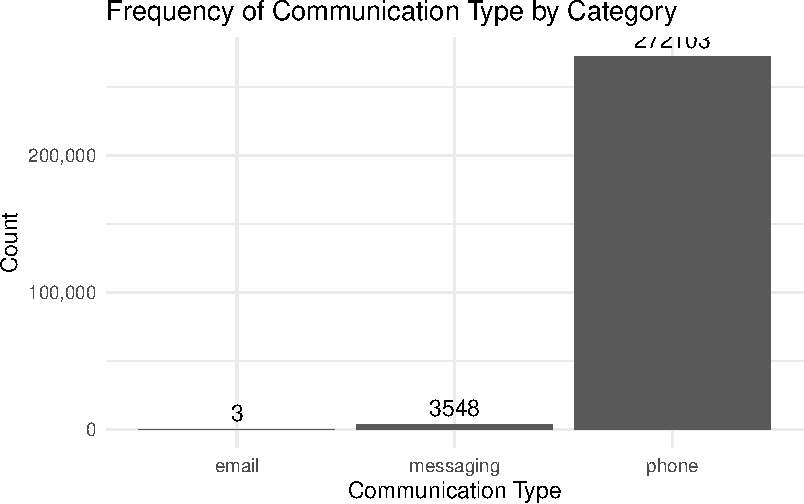
\includegraphics{final_proj_group1_files/figure-pdf/com_type-1.pdf}

\begin{Shaded}
\begin{Highlighting}[]
\NormalTok{df\_clean }\SpecialCharTok{\%\textgreater{}\%}
  \FunctionTok{count}\NormalTok{(SubCommunicationType) }\SpecialCharTok{\%\textgreater{}\%}
  \FunctionTok{ggplot}\NormalTok{(}\FunctionTok{aes}\NormalTok{(}\AttributeTok{x =}\NormalTok{ SubCommunicationType, }\AttributeTok{y =}\NormalTok{ n)) }\SpecialCharTok{+}
  \FunctionTok{geom\_bar}\NormalTok{(}\AttributeTok{stat =} \StringTok{"identity"}\NormalTok{) }\SpecialCharTok{+} 
  \FunctionTok{geom\_text}\NormalTok{(}\FunctionTok{aes}\NormalTok{(}\AttributeTok{label =}\NormalTok{ n), }\AttributeTok{vjust =} \SpecialCharTok{{-}}\FloatTok{0.5}\NormalTok{) }\SpecialCharTok{+}
  \FunctionTok{labs}\NormalTok{(}
    \AttributeTok{title =} \StringTok{"Frequency of Sub Communication Type by Category"}\NormalTok{,}
    \AttributeTok{x =} \StringTok{"Communication Type"}\NormalTok{, }
    \AttributeTok{y =} \StringTok{"Count"}
\NormalTok{  ) }\SpecialCharTok{+}
  \FunctionTok{scale\_y\_continuous}\NormalTok{(}\AttributeTok{labels =}\NormalTok{ comma) }\SpecialCharTok{+}
  \FunctionTok{theme\_minimal}\NormalTok{()}
\end{Highlighting}
\end{Shaded}

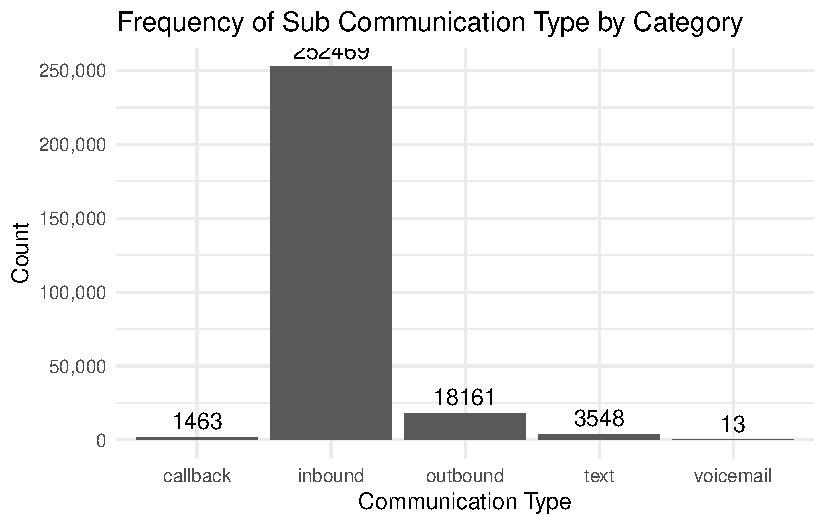
\includegraphics{final_proj_group1_files/figure-pdf/com_type-2.pdf}

\subsubsection{Observations}\label{observations}

Most communication type is by phone. Dataset contains mostly inbound
communication.

\subsection{Continuous Variables}\label{continuous-variables}

\begin{Shaded}
\begin{Highlighting}[]
\CommentTok{\# reshape data to long format}
\NormalTok{df\_long }\OtherTok{\textless{}{-}}\NormalTok{ df\_clean }\SpecialCharTok{\%\textgreater{}\%}
  \FunctionTok{pivot\_longer}\NormalTok{(}
    \AttributeTok{cols =} \FunctionTok{c}\NormalTok{(WaitTime, TimeInteracting, HoldTime, WrapUpTime), }
    \AttributeTok{names\_to =} \StringTok{"Variable"}\NormalTok{, }\AttributeTok{values\_to =} \StringTok{"Value"}
\NormalTok{  ) }\SpecialCharTok{\%\textgreater{}\%}
  \FunctionTok{mutate}\NormalTok{(}\AttributeTok{Value =}\NormalTok{ Value }\SpecialCharTok{/} \DecValTok{60}\NormalTok{)}

\CommentTok{\# create box plots}
\FunctionTok{ggplot}\NormalTok{(df\_long, }\FunctionTok{aes}\NormalTok{(}\AttributeTok{x =} \StringTok{""}\NormalTok{, }\AttributeTok{y =}\NormalTok{ Value)) }\SpecialCharTok{+} 
  \FunctionTok{geom\_boxplot}\NormalTok{() }\SpecialCharTok{+} 
  \FunctionTok{facet\_wrap}\NormalTok{(}\SpecialCharTok{\textasciitilde{}}\NormalTok{ Variable, }\AttributeTok{scales =} \StringTok{"free\_y"}\NormalTok{) }\SpecialCharTok{+} 
  \FunctionTok{coord\_cartesian}\NormalTok{(}\AttributeTok{ylim =} \FunctionTok{c}\NormalTok{(}\DecValTok{0}\NormalTok{, }\DecValTok{5}\NormalTok{)) }\SpecialCharTok{+}
  \FunctionTok{labs}\NormalTok{(}
    \AttributeTok{title =} \StringTok{"Distribution of Continuous Variables"}\NormalTok{, }
    \AttributeTok{x =} \StringTok{"Variable"}\NormalTok{, }
    \AttributeTok{y =} \StringTok{"Wait Time (minutes)"}
\NormalTok{  ) }\SpecialCharTok{+}
  \FunctionTok{scale\_y\_continuous}\NormalTok{( }\AttributeTok{labels =}\NormalTok{ comma ) }\SpecialCharTok{+}
  \FunctionTok{theme\_minimal}\NormalTok{()}
\end{Highlighting}
\end{Shaded}

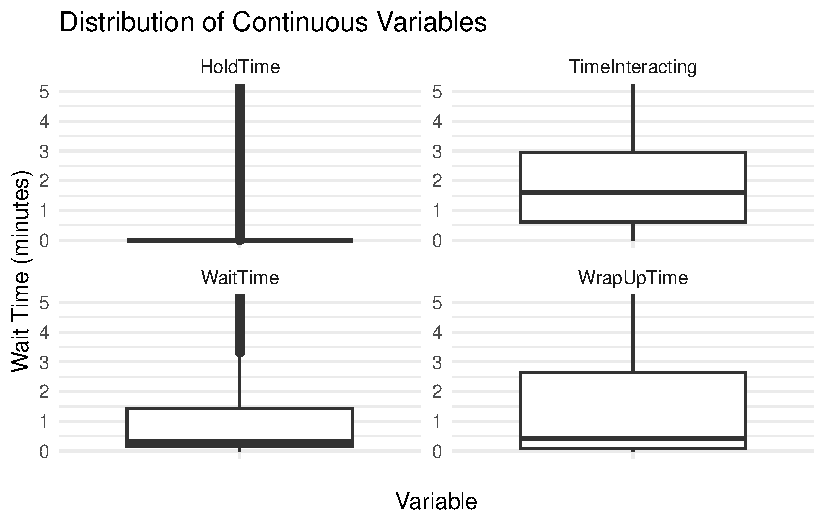
\includegraphics{final_proj_group1_files/figure-pdf/boxplot_contvar-1.pdf}

\begin{Shaded}
\begin{Highlighting}[]
\FunctionTok{ggplot}\NormalTok{(df\_long, }\FunctionTok{aes}\NormalTok{(}\AttributeTok{x =}\NormalTok{ Value)) }\SpecialCharTok{+}
  \FunctionTok{geom\_histogram}\NormalTok{(}\AttributeTok{bins =} \DecValTok{30}\NormalTok{, }\AttributeTok{fill =} \StringTok{"skyblue"}\NormalTok{, }\AttributeTok{color =} \StringTok{"black"}\NormalTok{) }\SpecialCharTok{+}
  \FunctionTok{facet\_wrap}\NormalTok{(}\SpecialCharTok{\textasciitilde{}}\NormalTok{ Variable, }\AttributeTok{scales =} \StringTok{"free\_x"}\NormalTok{) }\SpecialCharTok{+} 
  \FunctionTok{labs}\NormalTok{(}
    \AttributeTok{title =} \StringTok{"Distribution"}\NormalTok{,}
    \AttributeTok{x =} \StringTok{"Time (minutes)"}\NormalTok{, }
    \AttributeTok{y =} \StringTok{"Frequency"}
\NormalTok{  ) }\SpecialCharTok{+}
  \FunctionTok{scale\_y\_continuous}\NormalTok{(}\AttributeTok{labels =}\NormalTok{ comma) }\SpecialCharTok{+} 
  \FunctionTok{scale\_x\_continuous}\NormalTok{(}\AttributeTok{labels =}\NormalTok{ comma) }\SpecialCharTok{+} 
  \FunctionTok{theme\_minimal}\NormalTok{()}
\end{Highlighting}
\end{Shaded}

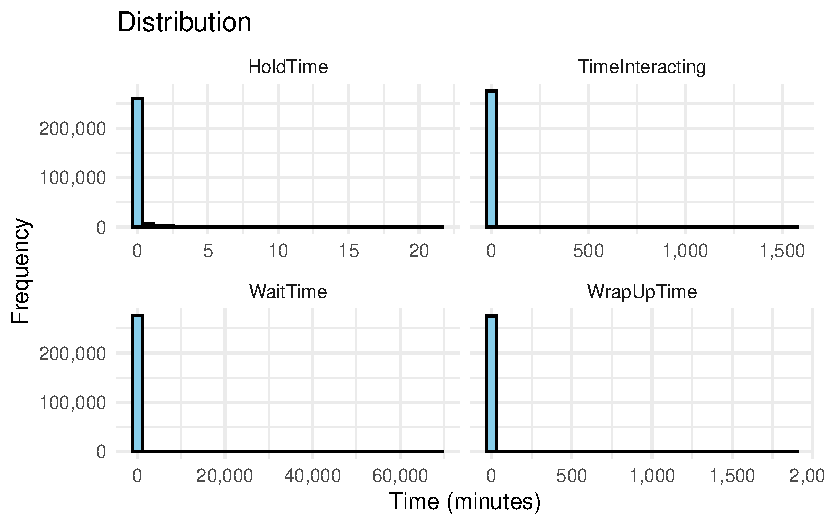
\includegraphics{final_proj_group1_files/figure-pdf/boxplot_contvar-2.pdf}

\begin{Shaded}
\begin{Highlighting}[]
\NormalTok{continuous\_var }\OtherTok{\textless{}{-}} \FunctionTok{c}\NormalTok{(}\StringTok{"WaitTime"}\NormalTok{, }\StringTok{"TimeInteracting"}\NormalTok{, }\StringTok{"HoldTime"}\NormalTok{, }\StringTok{"WrapUpTime"}\NormalTok{)}

\FunctionTok{skim}\NormalTok{(df\_clean[, continuous\_var]) }\SpecialCharTok{\%\textgreater{}\%}
  \FunctionTok{select}\NormalTok{(skim\_variable, numeric.mean, numeric.sd, numeric.p0, numeric.p25, numeric.p50, numeric.p75, numeric.p100) }\SpecialCharTok{\%\textgreater{}\%}
  \FunctionTok{gt}\NormalTok{() }\SpecialCharTok{\%\textgreater{}\%}
  \FunctionTok{fmt\_number}\NormalTok{(}
    \AttributeTok{columns =} \FunctionTok{everything}\NormalTok{(),}
    \AttributeTok{decimals =} \DecValTok{2}
\NormalTok{  ) }\SpecialCharTok{\%\textgreater{}\%}
  \FunctionTok{cols\_label}\NormalTok{(}
    \AttributeTok{skim\_variable =} \StringTok{"Variable"}\NormalTok{,}
    \AttributeTok{numeric.mean =} \StringTok{"Mean"}\NormalTok{, }
    \AttributeTok{numeric.sd =} \StringTok{"SD"}\NormalTok{, }
    \AttributeTok{numeric.p0 =} \StringTok{"Min"}\NormalTok{, }
    \AttributeTok{numeric.p25 =} \StringTok{"25\%"}\NormalTok{, }
    \AttributeTok{numeric.p50 =} \StringTok{"50\%"}\NormalTok{, }
    \AttributeTok{numeric.p75 =} \StringTok{"75\%"}\NormalTok{, }
    \AttributeTok{numeric.p100 =} \StringTok{"Max"}
\NormalTok{  ) }\SpecialCharTok{\%\textgreater{}\%}
  \FunctionTok{tab\_header}\NormalTok{(}
    \AttributeTok{title =} \StringTok{"Statistics for Continuous Variables (Minutes)"}
\NormalTok{  ) }\SpecialCharTok{\%\textgreater{}\%}
  \FunctionTok{tab\_style}\NormalTok{(}
    \AttributeTok{style =} \FunctionTok{cell\_text}\NormalTok{(}\AttributeTok{weight =} \StringTok{"bold"}\NormalTok{),}
    \AttributeTok{locations =} \FunctionTok{cells\_column\_labels}\NormalTok{(}\FunctionTok{everything}\NormalTok{())}
\NormalTok{  ) }\SpecialCharTok{\%\textgreater{}\%}
  \FunctionTok{cols\_align}\NormalTok{(}
    \AttributeTok{align =} \StringTok{"center"}\NormalTok{, }
    \AttributeTok{columns =} \FunctionTok{c}\NormalTok{(numeric.mean, numeric.sd, numeric.p0, numeric.p25, numeric.p50, numeric.p75, numeric.p100)}
\NormalTok{  )}
\end{Highlighting}
\end{Shaded}

\begin{table}
\caption*{
{\large Statistics for Continuous Variables (Minutes)}
} 
\fontsize{12.0pt}{14.4pt}\selectfont
\begin{tabular*}{\linewidth}{@{\extracolsep{\fill}}lccccccc}
\toprule
Variable & Mean & SD & Min & 25\% & 50\% & 75\% & Max \\ 
\midrule\addlinespace[2.5pt]
WaitTime & 118.69 & 7,975.21 & 0.00 & 10.00 & 18.00 & 86.00 & 4,126,179.00 \\ 
TimeInteracting & 132.02 & 303.75 & 0.00 & 37.00 & 96.00 & 177.00 & 93,296.00 \\ 
HoldTime & 6.32 & 34.76 & 0.00 & 0.00 & 0.00 & 0.00 & 1,284.00 \\ 
WrapUpTime & 141.40 & 1,034.73 & 0.00 & 5.00 & 25.00 & 159.00 & 112,600.00 \\ 
\bottomrule
\end{tabular*}
\end{table}

\subsubsection{Observations}\label{observations-1}

Each of the continuous variables have relatively low means and they also
contain extremely high outliers.

\subsection{Time Series}\label{time-series}

\subsubsection{Hourly}\label{hourly}

\begin{Shaded}
\begin{Highlighting}[]
\CommentTok{\# aggregate to hourly}
\NormalTok{df\_hourly }\OtherTok{\textless{}{-}}\NormalTok{ df\_clean }\SpecialCharTok{\%\textgreater{}\%}
  \FunctionTok{mutate}\NormalTok{(}\AttributeTok{hour =} \FunctionTok{floor\_date}\NormalTok{(StartTime, }\StringTok{"hour"}\NormalTok{)) }\SpecialCharTok{\%\textgreater{}\%}
  \FunctionTok{group\_by}\NormalTok{(hour) }\SpecialCharTok{\%\textgreater{}\%}
  \FunctionTok{summarise}\NormalTok{(}\AttributeTok{total\_calls =} \FunctionTok{n}\NormalTok{())}

\CommentTok{\# convert to tsibble}
\NormalTok{df\_hourly\_ts }\OtherTok{\textless{}{-}}\NormalTok{ df\_hourly }\SpecialCharTok{\%\textgreater{}\%}
  \FunctionTok{as\_tsibble}\NormalTok{(}\AttributeTok{index =}\NormalTok{ hour)}

\CommentTok{\# plot using autoplot}
\FunctionTok{autoplot}\NormalTok{(df\_hourly\_ts, total\_calls) }\SpecialCharTok{+}
  \FunctionTok{labs}\NormalTok{(}
    \AttributeTok{title =} \StringTok{"Total Calls by Hour over Time"}\NormalTok{, }
    \AttributeTok{x =} \StringTok{"Hour"}\NormalTok{,}
    \AttributeTok{y =} \StringTok{"Total Calls"}
\NormalTok{  ) }\SpecialCharTok{+}
  \FunctionTok{theme\_minimal}\NormalTok{()}
\end{Highlighting}
\end{Shaded}

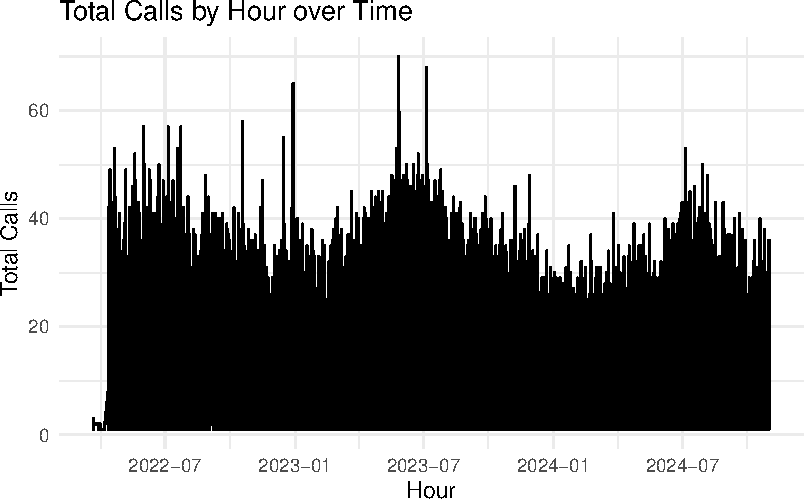
\includegraphics{final_proj_group1_files/figure-pdf/hourly-1.pdf}

\begin{Shaded}
\begin{Highlighting}[]
\CommentTok{\# distribution of calls by hour}
\FunctionTok{ggplot}\NormalTok{(df\_hourly, }\FunctionTok{aes}\NormalTok{(}\AttributeTok{x =}\NormalTok{ hour, }\AttributeTok{y =}\NormalTok{ total\_calls)) }\SpecialCharTok{+} 
  \FunctionTok{geom\_bar}\NormalTok{(}\AttributeTok{stat =} \StringTok{"identity"}\NormalTok{) }\SpecialCharTok{+}
  \FunctionTok{labs}\NormalTok{(}
    \AttributeTok{title =} \StringTok{"Distribution of Calls by Hour"}\NormalTok{, }
    \AttributeTok{x =} \StringTok{"Hour"}\NormalTok{, }
    \AttributeTok{y =} \StringTok{"Total Calls"}
\NormalTok{  )}
\end{Highlighting}
\end{Shaded}

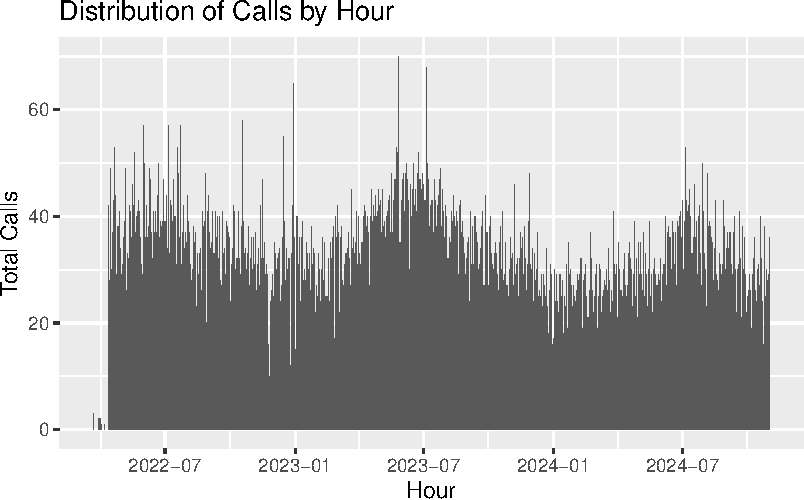
\includegraphics{final_proj_group1_files/figure-pdf/hourly-2.pdf}

\paragraph{Observations}\label{observations-2}

Time series at the hourly granularity is too noisy and visually
cluttered. Better information could be gathered at a lower frequency:
daily, weekly, or monthly.

\begin{Shaded}
\begin{Highlighting}[]
\CommentTok{\# aggregate to hour of day}
\NormalTok{df\_hour\_of\_day }\OtherTok{\textless{}{-}}\NormalTok{ df\_clean }\SpecialCharTok{\%\textgreater{}\%}
  \FunctionTok{mutate}\NormalTok{(}\AttributeTok{hour\_of\_day =} \FunctionTok{format}\NormalTok{(StartTime, }\StringTok{"\%H"}\NormalTok{)) }\SpecialCharTok{\%\textgreater{}\%}
  \FunctionTok{group\_by}\NormalTok{(hour\_of\_day) }\SpecialCharTok{\%\textgreater{}\%}
  \FunctionTok{summarise}\NormalTok{(}\AttributeTok{total\_calls =} \FunctionTok{n}\NormalTok{())}

\CommentTok{\# plot histogram of total counts}
\FunctionTok{ggplot}\NormalTok{(df\_hour\_of\_day, }\FunctionTok{aes}\NormalTok{(}\AttributeTok{x =}\NormalTok{ hour\_of\_day, }\AttributeTok{y =}\NormalTok{ total\_calls)) }\SpecialCharTok{+}
  \FunctionTok{geom\_bar}\NormalTok{(}\AttributeTok{stat =} \StringTok{"identity"}\NormalTok{, }\AttributeTok{fill =} \StringTok{"steelblue"}\NormalTok{) }\SpecialCharTok{+} 
  \FunctionTok{labs}\NormalTok{(}
    \AttributeTok{title =} \StringTok{"Distribution of Calls by Hour of Day"}\NormalTok{, }
    \AttributeTok{x =} \StringTok{"Hour of Day"}\NormalTok{, }
    \AttributeTok{y =} \StringTok{"Total Calls"}
\NormalTok{  ) }\SpecialCharTok{+}
  \FunctionTok{theme\_minimal}\NormalTok{()}
\end{Highlighting}
\end{Shaded}

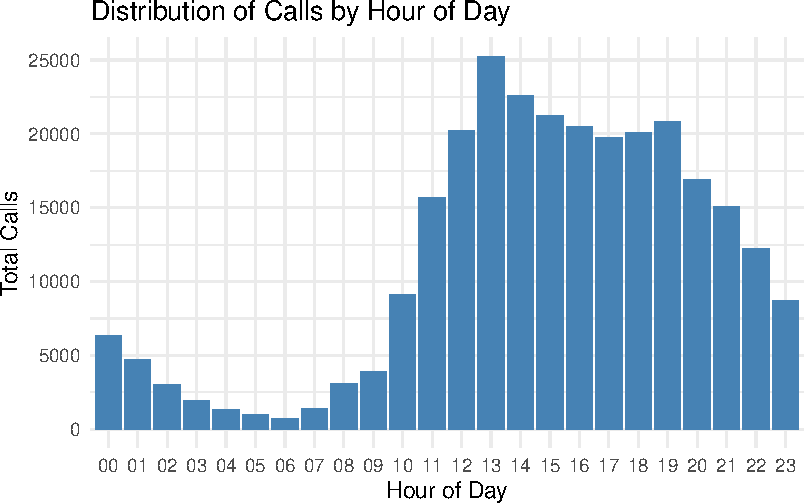
\includegraphics{final_proj_group1_files/figure-pdf/hour_of_day-1.pdf}

\begin{Shaded}
\begin{Highlighting}[]
\CommentTok{\# create df for median calls per hour}
\NormalTok{df\_daily\_hourly\_calls }\OtherTok{\textless{}{-}}\NormalTok{ df\_clean }\SpecialCharTok{\%\textgreater{}\%}
  \FunctionTok{mutate}\NormalTok{(}\AttributeTok{date =} \FunctionTok{as.Date}\NormalTok{(StartTime), }
         \AttributeTok{hour\_of\_day =} \FunctionTok{format}\NormalTok{(StartTime, }\StringTok{"\%H"}\NormalTok{)) }\SpecialCharTok{\%\textgreater{}\%}
  \FunctionTok{group\_by}\NormalTok{(date, hour\_of\_day) }\SpecialCharTok{\%\textgreater{}\%}
  \FunctionTok{summarise}\NormalTok{(}\AttributeTok{total\_calls =} \FunctionTok{n}\NormalTok{(), }\AttributeTok{.groups =} \StringTok{\textquotesingle{}drop\textquotesingle{}}\NormalTok{)}

\CommentTok{\# create df to calc median calls/hour}
\NormalTok{df\_hourly\_median }\OtherTok{\textless{}{-}}\NormalTok{ df\_daily\_hourly\_calls }\SpecialCharTok{\%\textgreater{}\%}
  \FunctionTok{group\_by}\NormalTok{(hour\_of\_day) }\SpecialCharTok{\%\textgreater{}\%}
  \FunctionTok{summarise}\NormalTok{(}\AttributeTok{median\_calls =} \FunctionTok{median}\NormalTok{(total\_calls), }\AttributeTok{.groups =} \StringTok{\textquotesingle{}drop\textquotesingle{}}\NormalTok{)}

\CommentTok{\# plot median calls by hour}
\FunctionTok{ggplot}\NormalTok{(df\_hourly\_median, }\FunctionTok{aes}\NormalTok{(}\AttributeTok{x =}\NormalTok{ hour\_of\_day, }\AttributeTok{y =}\NormalTok{ median\_calls)) }\SpecialCharTok{+} 
  \FunctionTok{geom\_bar}\NormalTok{(}\AttributeTok{stat =} \StringTok{"identity"}\NormalTok{, }\AttributeTok{fill =} \StringTok{"steelblue"}\NormalTok{) }\SpecialCharTok{+}
  \FunctionTok{labs}\NormalTok{(}
    \AttributeTok{title =} \StringTok{"Median Number of Calls by Hour of Day"}\NormalTok{, }
    \AttributeTok{x =} \StringTok{"Hour of Day"}\NormalTok{, }
    \AttributeTok{y =} \StringTok{"Median Calls"}
\NormalTok{  ) }\SpecialCharTok{+} 
  \FunctionTok{theme\_minimal}\NormalTok{()}
\end{Highlighting}
\end{Shaded}

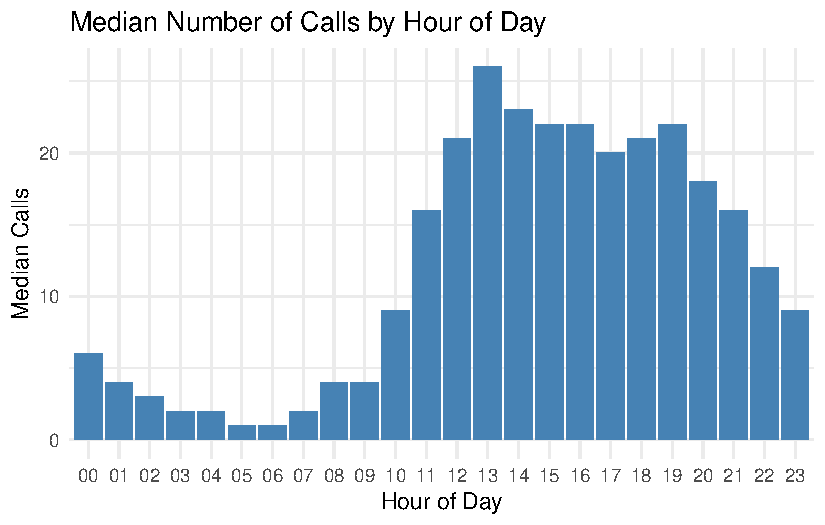
\includegraphics{final_proj_group1_files/figure-pdf/hour_of_day-2.pdf}

\paragraph{Observations}\label{observations-3}

Call volumes are greater than 15 calls/hour from 11am - 9pm.

\subsubsection{Daily}\label{daily}

\begin{Shaded}
\begin{Highlighting}[]
\CommentTok{\# aggregate to daily}
\NormalTok{df\_daily\_calls }\OtherTok{\textless{}{-}}\NormalTok{ df\_clean }\SpecialCharTok{\%\textgreater{}\%}
  \FunctionTok{mutate}\NormalTok{(}\AttributeTok{date =} \FunctionTok{as.Date}\NormalTok{(StartTime)) }\SpecialCharTok{\%\textgreater{}\%}
  \FunctionTok{group\_by}\NormalTok{(date) }\SpecialCharTok{\%\textgreater{}\%}
  \FunctionTok{summarise}\NormalTok{(}\AttributeTok{total\_calls =} \FunctionTok{n}\NormalTok{(), }\AttributeTok{.groups =} \StringTok{\textquotesingle{}drop\textquotesingle{}}\NormalTok{)}

\CommentTok{\# convert to tsibble}
\NormalTok{df\_daily\_calls\_ts }\OtherTok{\textless{}{-}}\NormalTok{ df\_daily\_calls }\SpecialCharTok{\%\textgreater{}\%}
  \FunctionTok{as\_tsibble}\NormalTok{(}\AttributeTok{index =}\NormalTok{ date)}

\CommentTok{\# plot time series of daily call vols}
\NormalTok{df\_daily\_calls\_ts }\SpecialCharTok{\%\textgreater{}\%}
  \FunctionTok{autoplot}\NormalTok{(total\_calls) }\SpecialCharTok{+} 
  \FunctionTok{labs}\NormalTok{(}
    \AttributeTok{title =} \StringTok{"Daily Call Volumes (Mar 2022 {-} Oct 2024)"}\NormalTok{,}
    \AttributeTok{y =} \StringTok{"Total Calls"}\NormalTok{,}
    \AttributeTok{x =} \StringTok{"Date"}
\NormalTok{  )}
\end{Highlighting}
\end{Shaded}

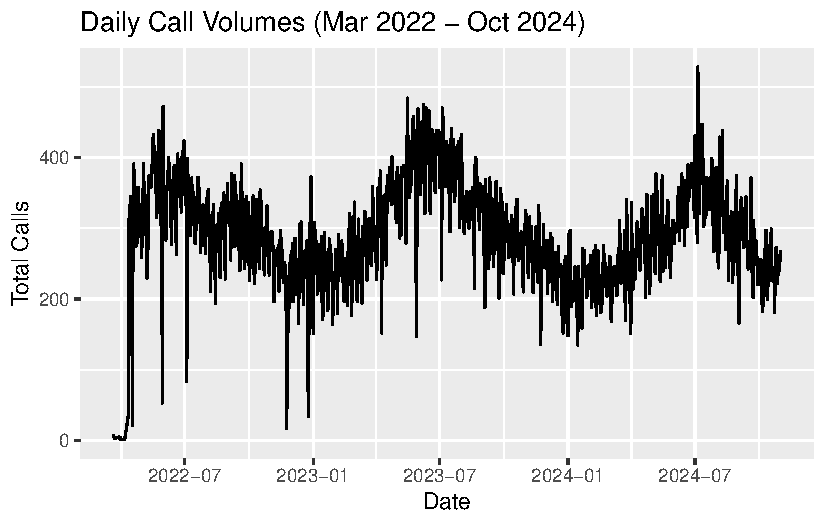
\includegraphics{final_proj_group1_files/figure-pdf/daily-1.pdf}

\begin{Shaded}
\begin{Highlighting}[]
\CommentTok{\# autocorrelation}
\NormalTok{df\_daily\_calls\_ts }\SpecialCharTok{\%\textgreater{}\%}
  \FunctionTok{fill\_gaps}\NormalTok{(}\AttributeTok{total\_calls =} \DecValTok{0}\NormalTok{) }\SpecialCharTok{\%\textgreater{}\%}
  \FunctionTok{ACF}\NormalTok{(total\_calls) }\SpecialCharTok{\%\textgreater{}\%}
  \FunctionTok{autoplot}\NormalTok{()}
\end{Highlighting}
\end{Shaded}

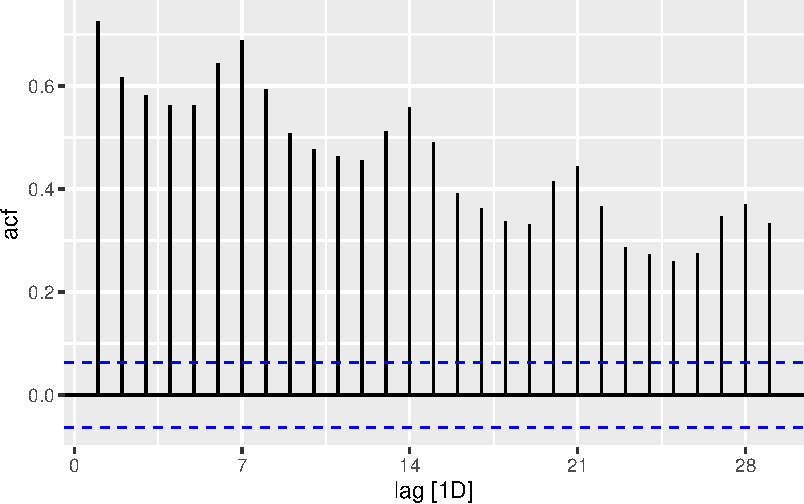
\includegraphics{final_proj_group1_files/figure-pdf/daily-2.pdf}

\begin{Shaded}
\begin{Highlighting}[]
\CommentTok{\# decomp of daily total call volume}
\NormalTok{decomp\_daily\_calls }\OtherTok{\textless{}{-}}\NormalTok{ df\_daily\_calls\_ts }\SpecialCharTok{\%\textgreater{}\%}
  \FunctionTok{fill\_gaps}\NormalTok{(}\AttributeTok{total\_calls =} \DecValTok{0}\NormalTok{) }\SpecialCharTok{\%\textgreater{}\%}
  \FunctionTok{model}\NormalTok{(}\AttributeTok{stl =} \FunctionTok{STL}\NormalTok{(total\_calls }\SpecialCharTok{\textasciitilde{}} \FunctionTok{season}\NormalTok{(}\AttributeTok{window =} \StringTok{"periodic"}\NormalTok{)))}

\CommentTok{\# extract and view decomp components}
\NormalTok{components\_calls\_daily }\OtherTok{\textless{}{-}}\NormalTok{ decomp\_daily\_calls }\SpecialCharTok{\%\textgreater{}\%}
  \FunctionTok{components}\NormalTok{()}

\CommentTok{\# plot decomp}
\NormalTok{components\_calls\_daily }\SpecialCharTok{\%\textgreater{}\%}
  \FunctionTok{autoplot}\NormalTok{() }\SpecialCharTok{+}
  \FunctionTok{labs}\NormalTok{(}
    \AttributeTok{title =} \StringTok{"STL Decomposition of Daily Call Volumes"}\NormalTok{, }
    \AttributeTok{y =} \StringTok{"Total Calls"}\NormalTok{, }
    \AttributeTok{x =} \StringTok{"Date"}
\NormalTok{  )}
\end{Highlighting}
\end{Shaded}

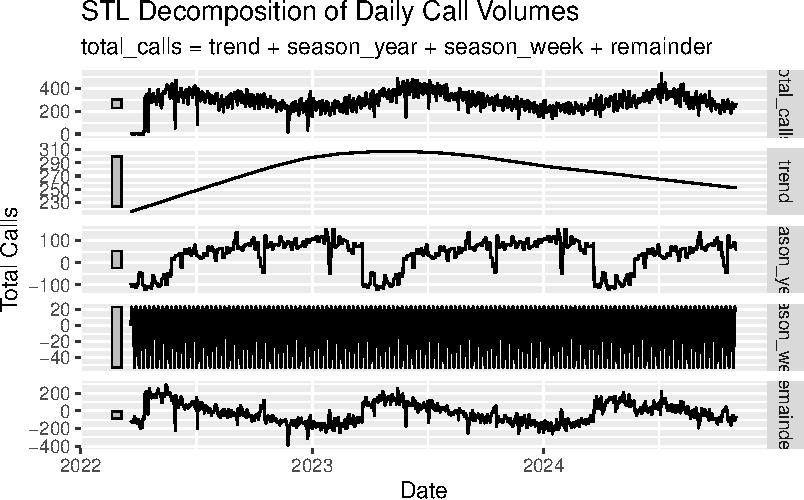
\includegraphics{final_proj_group1_files/figure-pdf/daily-3.pdf}

\paragraph{Observations}\label{observations-4}

These plots suggest a seasonal pattern in call volumes.

The ACF plot suggests strong autocorrelation with weekly seasonality as
seen in the spikes every 7 days.

\begin{Shaded}
\begin{Highlighting}[]
\CommentTok{\# create var for day of week order}
\NormalTok{days\_of\_week\_order }\OtherTok{=} \FunctionTok{c}\NormalTok{(}\StringTok{"Sunday"}\NormalTok{, }\StringTok{"Monday"}\NormalTok{, }\StringTok{"Tuesday"}\NormalTok{, }\StringTok{"Wednesday"}\NormalTok{, }\StringTok{"Thursday"}\NormalTok{, }\StringTok{"Friday"}\NormalTok{, }\StringTok{"Saturday"}\NormalTok{)}

\CommentTok{\# aggregate median calls by date }
\NormalTok{df\_median\_calls\_by\_day }\OtherTok{\textless{}{-}}\NormalTok{ df\_daily\_calls }\SpecialCharTok{\%\textgreater{}\%}
  \FunctionTok{mutate}\NormalTok{(}\AttributeTok{day\_of\_week =} \FunctionTok{weekdays}\NormalTok{(date)) }\SpecialCharTok{\%\textgreater{}\%}
  \FunctionTok{group\_by}\NormalTok{(day\_of\_week) }\SpecialCharTok{\%\textgreater{}\%}
  \FunctionTok{summarise}\NormalTok{(}\AttributeTok{median\_calls =} \FunctionTok{median}\NormalTok{(total\_calls), }\AttributeTok{.groups =} \StringTok{\textquotesingle{}drop\textquotesingle{}}\NormalTok{)}

\CommentTok{\# factor to ensure proper day of week order}
\NormalTok{df\_median\_calls\_by\_day}\SpecialCharTok{$}\NormalTok{day\_of\_week }\OtherTok{\textless{}{-}} \FunctionTok{factor}\NormalTok{(}
\NormalTok{  df\_median\_calls\_by\_day}\SpecialCharTok{$}\NormalTok{day\_of\_week, }
  \AttributeTok{levels =}\NormalTok{ days\_of\_week\_order}
\NormalTok{)}

\CommentTok{\# }
\NormalTok{df\_median\_calls\_by\_day }\SpecialCharTok{\%\textgreater{}\%}
  \FunctionTok{ggplot}\NormalTok{(}\FunctionTok{aes}\NormalTok{(}\AttributeTok{x =}\NormalTok{ day\_of\_week, }\AttributeTok{y =}\NormalTok{ median\_calls)) }\SpecialCharTok{+} 
  \FunctionTok{geom\_bar}\NormalTok{(}\AttributeTok{stat =} \StringTok{"identity"}\NormalTok{, }\AttributeTok{fill =} \StringTok{"steelblue"}\NormalTok{) }\SpecialCharTok{+}
  \FunctionTok{labs}\NormalTok{(}
    \AttributeTok{title =} \StringTok{"Median Number of Calls by Day of the Week"}\NormalTok{, }
    \AttributeTok{x =} \StringTok{"Day of the Week"}\NormalTok{, }
    \AttributeTok{y =} \StringTok{"Median Calls"}
\NormalTok{  ) }\SpecialCharTok{+}
  \FunctionTok{theme\_minimal}\NormalTok{()}
\end{Highlighting}
\end{Shaded}

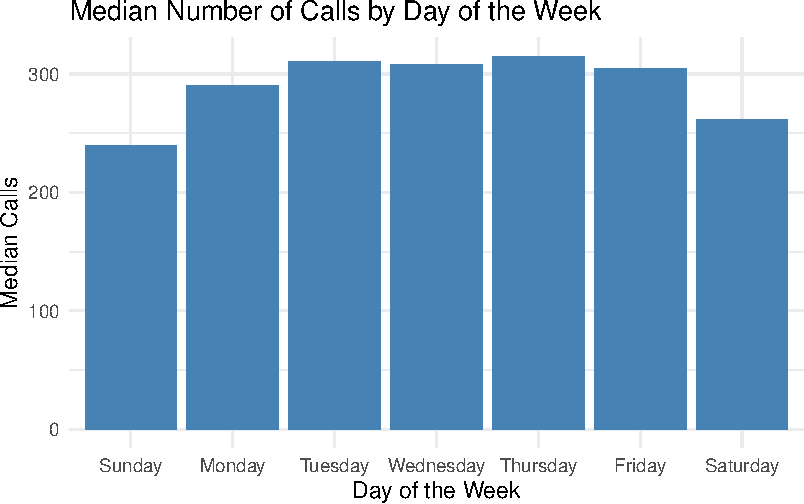
\includegraphics{final_proj_group1_files/figure-pdf/day_of_wk_dist-1.pdf}

\begin{Shaded}
\begin{Highlighting}[]
\CommentTok{\# df group by day of week and hour of day}
\NormalTok{df\_day\_hour\_calls }\OtherTok{\textless{}{-}}\NormalTok{ df\_clean }\SpecialCharTok{\%\textgreater{}\%}
  \FunctionTok{mutate}\NormalTok{(}\AttributeTok{day\_of\_week =} \FunctionTok{weekdays}\NormalTok{(}\FunctionTok{as.Date}\NormalTok{(StartTime)),}
         \AttributeTok{hour\_of\_day =} \FunctionTok{format}\NormalTok{(StartTime, }\StringTok{"\%H"}\NormalTok{)) }\SpecialCharTok{\%\textgreater{}\%}
  \FunctionTok{group\_by}\NormalTok{(day\_of\_week, hour\_of\_day) }\SpecialCharTok{\%\textgreater{}\%}
  \FunctionTok{summarise}\NormalTok{(}\AttributeTok{total\_calls =} \FunctionTok{n}\NormalTok{(), }\AttributeTok{.groups =} \StringTok{\textquotesingle{}drop\textquotesingle{}}\NormalTok{)}

\CommentTok{\# factor for day of week order}
\NormalTok{df\_day\_hour\_calls}\SpecialCharTok{$}\NormalTok{day\_of\_week }\OtherTok{\textless{}{-}} \FunctionTok{factor}\NormalTok{(}
\NormalTok{  df\_day\_hour\_calls}\SpecialCharTok{$}\NormalTok{day\_of\_week,}
  \AttributeTok{levels =}\NormalTok{ days\_of\_week\_order}
\NormalTok{)}

\CommentTok{\# plot heatmap}
\NormalTok{df\_day\_hour\_calls }\SpecialCharTok{\%\textgreater{}\%}
  \FunctionTok{ggplot}\NormalTok{(}\FunctionTok{aes}\NormalTok{(}\AttributeTok{x =}\NormalTok{ hour\_of\_day, }\AttributeTok{y =}\NormalTok{ day\_of\_week, }\AttributeTok{fill =}\NormalTok{ total\_calls)) }\SpecialCharTok{+}
  \FunctionTok{geom\_tile}\NormalTok{() }\SpecialCharTok{+}
  \FunctionTok{scale\_fill\_gradient}\NormalTok{(}\AttributeTok{low =} \StringTok{"lightblue"}\NormalTok{, }\AttributeTok{high =} \StringTok{"darkblue"}\NormalTok{) }\SpecialCharTok{+}
  \FunctionTok{labs}\NormalTok{(}
    \AttributeTok{title =} \StringTok{"Heat Map of Call Volumes by Day of Week and Hour of Day"}\NormalTok{, }
    \AttributeTok{x =} \StringTok{"Hour of Day"}\NormalTok{, }
    \AttributeTok{y =} \StringTok{"Day of Week"}\NormalTok{, }
    \AttributeTok{fill =} \StringTok{"Total Calls"}
\NormalTok{  ) }\SpecialCharTok{+}
  \FunctionTok{theme\_minimal}\NormalTok{()}
\end{Highlighting}
\end{Shaded}

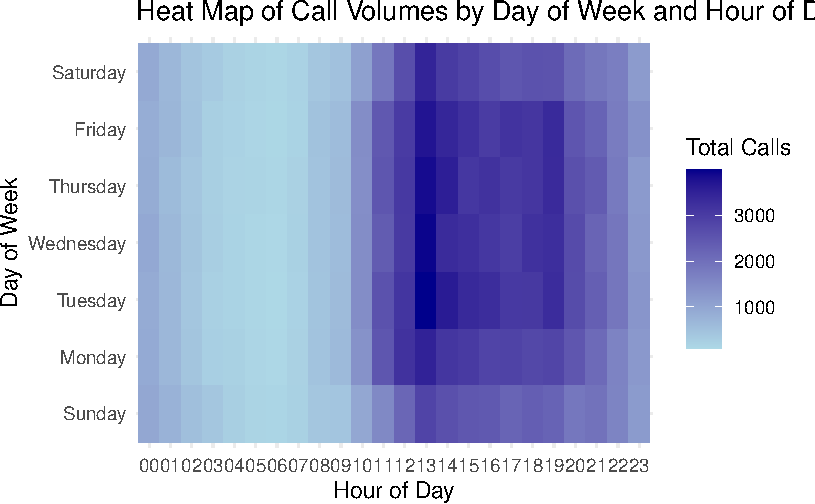
\includegraphics{final_proj_group1_files/figure-pdf/day_vs_hour-1.pdf}

\paragraph{Observations}\label{observations-5}

Call volumes are highest, exceeding 300 calls per day from Tuesday
through Friday and mostly concentrated around 1300 hrs.

\subsubsection{Weekly - Total Call
Volume}\label{weekly---total-call-volume}

\begin{Shaded}
\begin{Highlighting}[]
\NormalTok{df\_weekly }\OtherTok{\textless{}{-}}\NormalTok{ df\_clean }\SpecialCharTok{\%\textgreater{}\%}
  \FunctionTok{mutate}\NormalTok{(}\AttributeTok{week =} \FunctionTok{floor\_date}\NormalTok{(}\FunctionTok{as.Date}\NormalTok{(StartTime), }\StringTok{"week"}\NormalTok{)) }\SpecialCharTok{\%\textgreater{}\%}  \CommentTok{\# Round StartTime to the beginning of the week}
  \FunctionTok{group\_by}\NormalTok{(week) }\SpecialCharTok{\%\textgreater{}\%}
  \FunctionTok{summarise}\NormalTok{(}\AttributeTok{total\_calls =} \FunctionTok{n}\NormalTok{()) }\SpecialCharTok{\%\textgreater{}\%}  \CommentTok{\# Count the number of rows (calls) per week}
  \FunctionTok{ungroup}\NormalTok{() }\SpecialCharTok{\%\textgreater{}\%}
  \CommentTok{\# Fill in missing weeks with 0 calls}
  \FunctionTok{complete}\NormalTok{(}\AttributeTok{week =} \FunctionTok{seq.Date}\NormalTok{(}\FunctionTok{min}\NormalTok{(week), }\FunctionTok{max}\NormalTok{(week), }\AttributeTok{by =} \StringTok{"week"}\NormalTok{), }\AttributeTok{fill =} \FunctionTok{list}\NormalTok{(}\AttributeTok{total\_calls =} \DecValTok{0}\NormalTok{))  }

\NormalTok{df\_weekly\_ts }\OtherTok{\textless{}{-}}\NormalTok{ df\_weekly }\SpecialCharTok{\%\textgreater{}\%}
  \FunctionTok{as\_tsibble}\NormalTok{(}\AttributeTok{index =}\NormalTok{ week)}

\CommentTok{\# plot chart}
\NormalTok{df\_weekly\_ts }\SpecialCharTok{\%\textgreater{}\%}
  \FunctionTok{autoplot}\NormalTok{(total\_calls) }\SpecialCharTok{+}
  \FunctionTok{labs}\NormalTok{(}
    \AttributeTok{title =} \StringTok{"Weekly Call Volumes (Mar 2022 {-} Oct 2024)"}\NormalTok{,}
    \AttributeTok{y =} \StringTok{"Total Calls"}\NormalTok{,}
    \AttributeTok{x =} \StringTok{"Date"}
\NormalTok{  ) }\SpecialCharTok{+} 
  \FunctionTok{theme\_minimal}\NormalTok{()}
\end{Highlighting}
\end{Shaded}

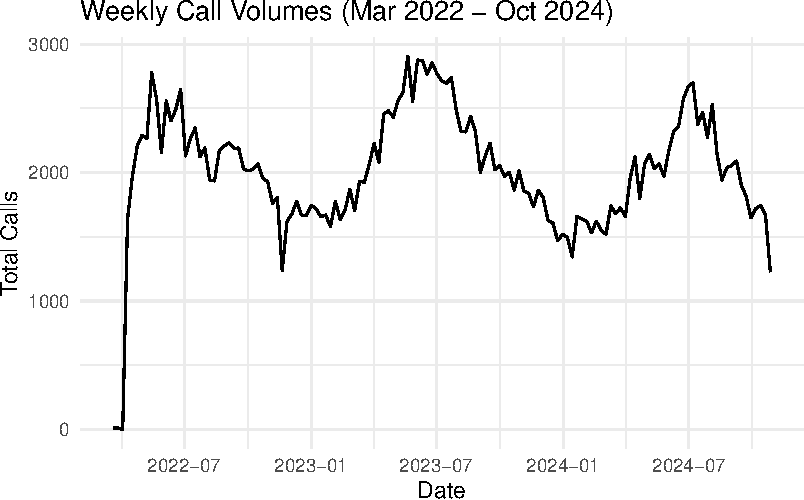
\includegraphics{final_proj_group1_files/figure-pdf/weekly-1.pdf}

\begin{Shaded}
\begin{Highlighting}[]
\CommentTok{\# autocorrelation}
\NormalTok{df\_weekly\_ts }\SpecialCharTok{\%\textgreater{}\%}
  \FunctionTok{ACF}\NormalTok{(total\_calls) }\SpecialCharTok{\%\textgreater{}\%}
  \FunctionTok{autoplot}\NormalTok{()}
\end{Highlighting}
\end{Shaded}

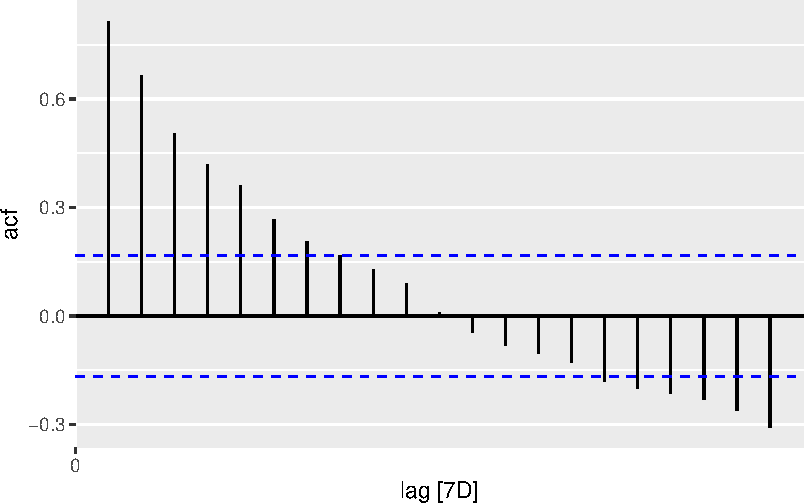
\includegraphics{final_proj_group1_files/figure-pdf/weekly-2.pdf}

\begin{Shaded}
\begin{Highlighting}[]
\CommentTok{\# decomp of weekly total call volume}
\NormalTok{decomp\_calls }\OtherTok{\textless{}{-}}\NormalTok{ df\_weekly\_ts }\SpecialCharTok{\%\textgreater{}\%}
  \FunctionTok{fill\_gaps}\NormalTok{(}\AttributeTok{total\_calls =} \DecValTok{0}\NormalTok{) }\SpecialCharTok{\%\textgreater{}\%}
  \FunctionTok{model}\NormalTok{(}\AttributeTok{stl =} \FunctionTok{STL}\NormalTok{(total\_calls }\SpecialCharTok{\textasciitilde{}} \FunctionTok{season}\NormalTok{(}\AttributeTok{window =} \StringTok{"periodic"}\NormalTok{)))}

\CommentTok{\# extract and view decomp components}
\NormalTok{components\_calls }\OtherTok{\textless{}{-}}\NormalTok{ decomp\_calls }\SpecialCharTok{\%\textgreater{}\%}
  \FunctionTok{components}\NormalTok{()}

\CommentTok{\# plot decomp}
\NormalTok{components\_calls }\SpecialCharTok{\%\textgreater{}\%}
  \FunctionTok{autoplot}\NormalTok{() }\SpecialCharTok{+}
  \FunctionTok{labs}\NormalTok{(}
    \AttributeTok{title =} \StringTok{"STL Decomposition of Weekly Call Volumes"}\NormalTok{, }
    \AttributeTok{y =} \StringTok{"Total Calls"}\NormalTok{, }
    \AttributeTok{x =} \StringTok{"Date"}
\NormalTok{  ) }\SpecialCharTok{+}
  \FunctionTok{theme\_minimal}\NormalTok{()}
\end{Highlighting}
\end{Shaded}

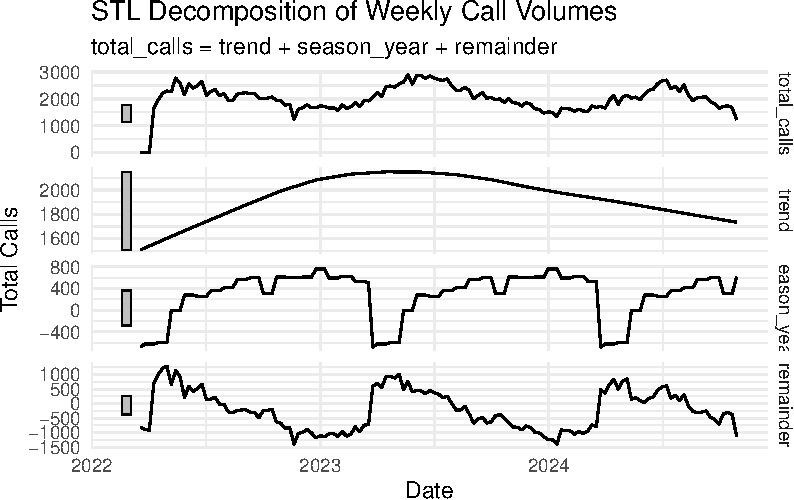
\includegraphics{final_proj_group1_files/figure-pdf/weekly-3.pdf}

\paragraph{Observations}\label{observations-6}

These chart shows that weekly call volumes may be seasonal. The ACF
chart suggests there is significant positive autocorrelation.

The Remainder chart does not appear to be random. This would need to be
explored further to determine if there are any uncaptured season trends.

\subsubsection{Monthly}\label{monthly}

\begin{Shaded}
\begin{Highlighting}[]
\CommentTok{\# aggregate by month}
\NormalTok{df\_monthly\_calls }\OtherTok{\textless{}{-}}\NormalTok{ df\_clean }\SpecialCharTok{\%\textgreater{}\%}
  \FunctionTok{mutate}\NormalTok{(}\AttributeTok{month =} \FunctionTok{floor\_date}\NormalTok{(}\FunctionTok{as.Date}\NormalTok{(StartTime), }\StringTok{"month"}\NormalTok{)) }\SpecialCharTok{\%\textgreater{}\%}
  \FunctionTok{group\_by}\NormalTok{(month) }\SpecialCharTok{\%\textgreater{}\%}
  \FunctionTok{summarise}\NormalTok{(}\AttributeTok{total\_calls =} \FunctionTok{n}\NormalTok{(), }\AttributeTok{.groups =} \StringTok{\textquotesingle{}drop\textquotesingle{}}\NormalTok{)}

\CommentTok{\# convert to tsibble}
\NormalTok{df\_monthly\_calls\_ts }\OtherTok{\textless{}{-}}\NormalTok{ df\_monthly\_calls }\SpecialCharTok{\%\textgreater{}\%}
  \FunctionTok{as\_tsibble}\NormalTok{(}\AttributeTok{index =}\NormalTok{ month)}

\CommentTok{\# plot}
\NormalTok{df\_monthly\_calls\_ts }\SpecialCharTok{\%\textgreater{}\%}
  \FunctionTok{autoplot}\NormalTok{(total\_calls) }\SpecialCharTok{+}
  \FunctionTok{labs}\NormalTok{(}
    \AttributeTok{title =} \StringTok{"Monthly Call Volumes (Mar 2022 {-} Oct 2024)"}\NormalTok{, }
    \AttributeTok{y =} \StringTok{"Total Calls"}\NormalTok{, }
    \AttributeTok{x =} \StringTok{"Date"}
\NormalTok{  ) }\SpecialCharTok{+} 
  \FunctionTok{theme\_minimal}\NormalTok{() }
\end{Highlighting}
\end{Shaded}

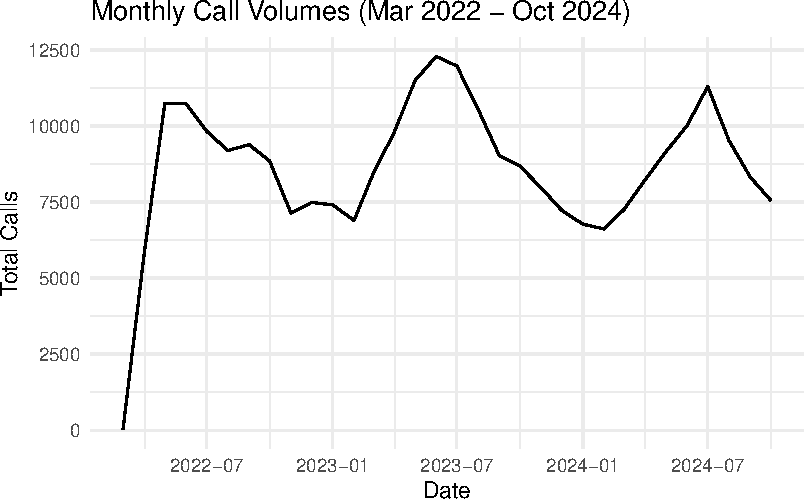
\includegraphics{final_proj_group1_files/figure-pdf/unnamed-chunk-1-1.pdf}

\begin{Shaded}
\begin{Highlighting}[]
\CommentTok{\# plot autocorrelation}
\NormalTok{df\_monthly\_calls\_ts }\SpecialCharTok{\%\textgreater{}\%}
  \FunctionTok{fill\_gaps}\NormalTok{(}\AttributeTok{total\_calls =} \DecValTok{0}\NormalTok{) }\SpecialCharTok{\%\textgreater{}\%}
  \FunctionTok{ACF}\NormalTok{(total\_calls) }\SpecialCharTok{\%\textgreater{}\%}
  \FunctionTok{autoplot}\NormalTok{() }\SpecialCharTok{+} 
  \FunctionTok{labs}\NormalTok{(}
    \AttributeTok{title =} \StringTok{"ACF of Monthly Call Volumes Time Series"}\NormalTok{,}
    \AttributeTok{y =} \StringTok{"Autocorrelation"}
\NormalTok{  )}
\end{Highlighting}
\end{Shaded}

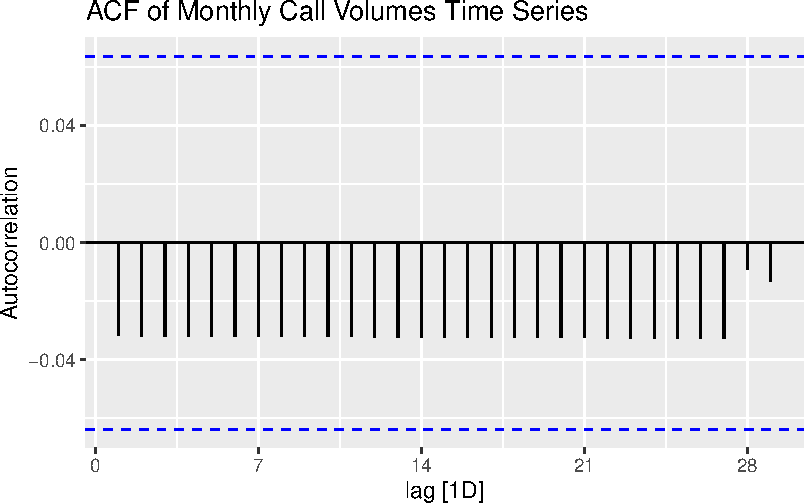
\includegraphics{final_proj_group1_files/figure-pdf/unnamed-chunk-1-2.pdf}

\begin{Shaded}
\begin{Highlighting}[]
\CommentTok{\# decomp of weekly total call volume}
\NormalTok{decomp\_calls\_monthly }\OtherTok{\textless{}{-}}\NormalTok{ df\_monthly\_calls\_ts }\SpecialCharTok{\%\textgreater{}\%}
  \FunctionTok{fill\_gaps}\NormalTok{(}\AttributeTok{total\_calls =} \DecValTok{0}\NormalTok{) }\SpecialCharTok{\%\textgreater{}\%}
  \FunctionTok{model}\NormalTok{(}\AttributeTok{stl =} \FunctionTok{STL}\NormalTok{(total\_calls }\SpecialCharTok{\textasciitilde{}} \FunctionTok{season}\NormalTok{(}\AttributeTok{window =} \StringTok{"periodic"}\NormalTok{)))}

\CommentTok{\# extract and view decomp components}
\NormalTok{components\_calls\_monthly }\OtherTok{\textless{}{-}}\NormalTok{ decomp\_calls\_monthly }\SpecialCharTok{\%\textgreater{}\%}
  \FunctionTok{components}\NormalTok{()}

\CommentTok{\# plot decomp}
\NormalTok{components\_calls\_monthly }\SpecialCharTok{\%\textgreater{}\%}
  \FunctionTok{autoplot}\NormalTok{() }\SpecialCharTok{+}
  \FunctionTok{labs}\NormalTok{(}
    \AttributeTok{title =} \StringTok{"STL Decomposition of Monthly Call Volumes"}\NormalTok{, }
    \AttributeTok{y =} \StringTok{"Total Calls"}\NormalTok{, }
    \AttributeTok{x =} \StringTok{"Date"}
\NormalTok{  ) }\SpecialCharTok{+}
  \FunctionTok{theme\_minimal}\NormalTok{()}
\end{Highlighting}
\end{Shaded}

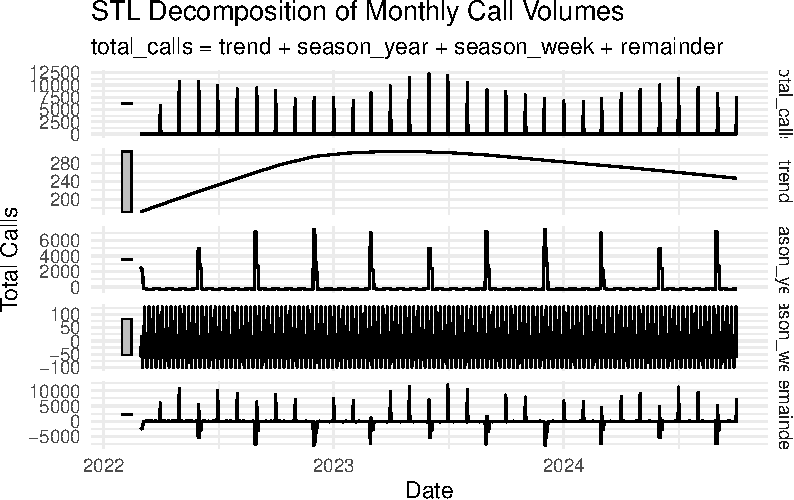
\includegraphics{final_proj_group1_files/figure-pdf/unnamed-chunk-1-3.pdf}

\paragraph{Observations}\label{observations-7}

Monthly call volumes appear to have seasonal pattern. The ACF chart
shows that there are no lags outside of the significance threshold
indicating low autocorrelation.

\begin{Shaded}
\begin{Highlighting}[]
\CommentTok{\# aggregate by month}
\NormalTok{df\_median\_calls\_by\_month }\OtherTok{\textless{}{-}}\NormalTok{ df\_daily\_calls }\SpecialCharTok{\%\textgreater{}\%}
  \FunctionTok{mutate}\NormalTok{(}\AttributeTok{month =} \FunctionTok{month}\NormalTok{(date, }\AttributeTok{label =} \ConstantTok{TRUE}\NormalTok{, }\AttributeTok{abbr =} \ConstantTok{FALSE}\NormalTok{)) }\SpecialCharTok{\%\textgreater{}\%}
  \FunctionTok{group\_by}\NormalTok{(month) }\SpecialCharTok{\%\textgreater{}\%}
  \FunctionTok{summarise}\NormalTok{(}\AttributeTok{median\_calls =} \FunctionTok{median}\NormalTok{(total\_calls), }\AttributeTok{.groups =} \StringTok{"drop"}\NormalTok{)}

\CommentTok{\# plot }
\NormalTok{df\_median\_calls\_by\_month }\SpecialCharTok{\%\textgreater{}\%}
  \FunctionTok{ggplot}\NormalTok{(}\FunctionTok{aes}\NormalTok{(}\AttributeTok{x =}\NormalTok{ month, }\AttributeTok{y =}\NormalTok{ median\_calls)) }\SpecialCharTok{+} 
  \FunctionTok{geom\_bar}\NormalTok{(}\AttributeTok{stat =} \StringTok{"identity"}\NormalTok{, }\AttributeTok{fill =} \StringTok{"steelblue"}\NormalTok{) }\SpecialCharTok{+}
  \FunctionTok{labs}\NormalTok{(}
    \AttributeTok{title =} \StringTok{"Median Calls by Month"}\NormalTok{, }
    \AttributeTok{x =} \StringTok{"Month"}\NormalTok{, }
    \AttributeTok{y =} \StringTok{"Median Calls"}
\NormalTok{  ) }\SpecialCharTok{+} \FunctionTok{theme\_minimal}\NormalTok{()}
\end{Highlighting}
\end{Shaded}

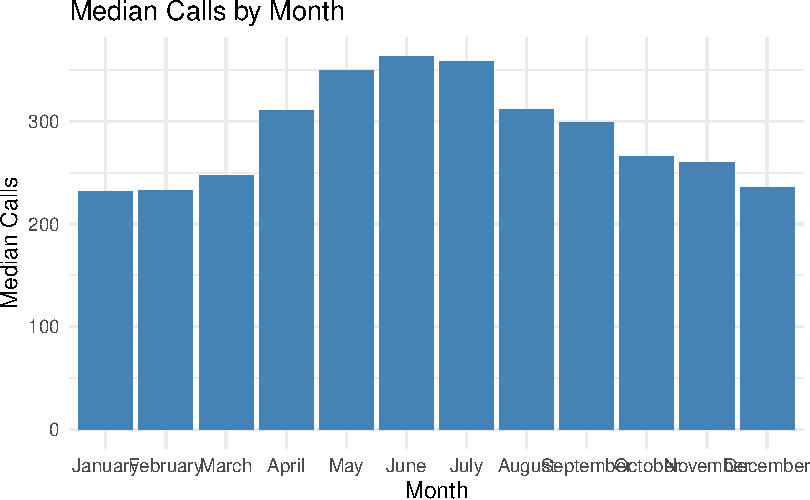
\includegraphics{final_proj_group1_files/figure-pdf/unnamed-chunk-2-1.pdf}

\paragraph{Observations}\label{observations-8}

Median call volumes \textgreater{} 300 call occur between April -
August.

\subsubsection{Weekly - Average of
WaitTime}\label{weekly---average-of-waittime}

\begin{Shaded}
\begin{Highlighting}[]
\NormalTok{df\_weekly\_wait }\OtherTok{\textless{}{-}}\NormalTok{ df\_clean }\SpecialCharTok{\%\textgreater{}\%}
  \FunctionTok{mutate}\NormalTok{(}\AttributeTok{week =} \FunctionTok{floor\_date}\NormalTok{(}\FunctionTok{as.Date}\NormalTok{(StartTime), }\StringTok{"week"}\NormalTok{)) }\SpecialCharTok{\%\textgreater{}\%}
  \FunctionTok{group\_by}\NormalTok{(week) }\SpecialCharTok{\%\textgreater{}\%}
  \FunctionTok{summarise}\NormalTok{(}\AttributeTok{avg\_wait\_time =} \FunctionTok{mean}\NormalTok{(WaitTime, }\AttributeTok{na.rm =} \ConstantTok{TRUE}\NormalTok{)) }\SpecialCharTok{\%\textgreater{}\%}
  \FunctionTok{ungroup}\NormalTok{() }\SpecialCharTok{\%\textgreater{}\%}
  \CommentTok{\# Fill in missing weeks}
  \FunctionTok{complete}\NormalTok{(}\AttributeTok{week =} \FunctionTok{seq.Date}\NormalTok{(}\FunctionTok{min}\NormalTok{(week), }\FunctionTok{max}\NormalTok{(week), }\AttributeTok{by =} \StringTok{"week"}\NormalTok{), }\AttributeTok{fill =} \FunctionTok{list}\NormalTok{(}\AttributeTok{avg\_wait\_time =} \DecValTok{0}\NormalTok{))}

\CommentTok{\# convert to tsibble}
\NormalTok{df\_weekly\_wait\_ts }\OtherTok{\textless{}{-}}\NormalTok{ df\_weekly\_wait }\SpecialCharTok{\%\textgreater{}\%}
  \FunctionTok{as\_tsibble}\NormalTok{(}\AttributeTok{index =}\NormalTok{ week)}

\CommentTok{\# plot chart}
\NormalTok{df\_weekly\_wait\_ts }\SpecialCharTok{\%\textgreater{}\%}
  \FunctionTok{autoplot}\NormalTok{(avg\_wait\_time) }\SpecialCharTok{+}
  \FunctionTok{labs}\NormalTok{(}
    \AttributeTok{title =} \StringTok{"Weekly Average Wait Time (Mar 2022 {-} Oct 2024)"}\NormalTok{, }
    \AttributeTok{y =} \StringTok{"Average Wait Time (min)"}\NormalTok{,}
    \AttributeTok{x =} \StringTok{"Date"}
\NormalTok{  ) }\SpecialCharTok{+}
  \FunctionTok{theme\_minimal}\NormalTok{()}
\end{Highlighting}
\end{Shaded}

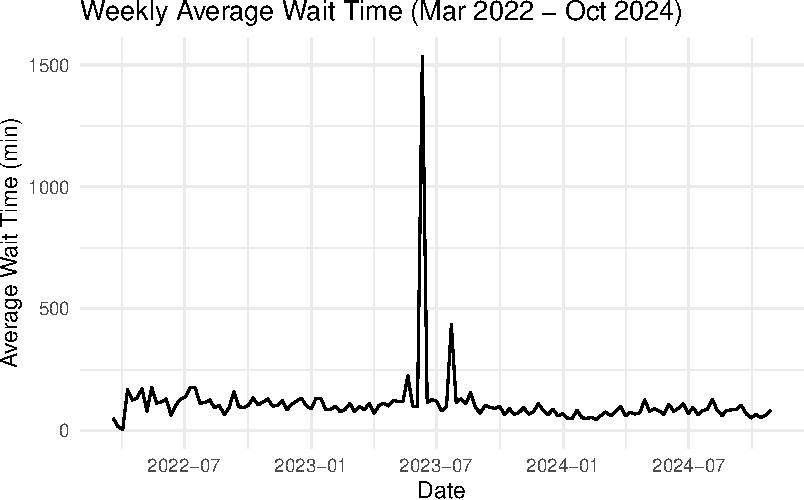
\includegraphics{final_proj_group1_files/figure-pdf/unnamed-chunk-3-1.pdf}

\begin{Shaded}
\begin{Highlighting}[]
\CommentTok{\# autocorrelation}
\NormalTok{df\_weekly\_wait\_ts }\SpecialCharTok{\%\textgreater{}\%}
  \FunctionTok{fill\_gaps}\NormalTok{(}\AttributeTok{avg\_wait\_time =} \DecValTok{0}\NormalTok{) }\SpecialCharTok{\%\textgreater{}\%}
  \FunctionTok{ACF}\NormalTok{(avg\_wait\_time) }\SpecialCharTok{\%\textgreater{}\%}
  \FunctionTok{autoplot}\NormalTok{() }\SpecialCharTok{+} 
  \FunctionTok{labs}\NormalTok{(}
    \AttributeTok{title =} \StringTok{"ACF of Weekly Average Wait Time"}\NormalTok{, }
    \AttributeTok{y =} \StringTok{"ACF"}
\NormalTok{  )}
\end{Highlighting}
\end{Shaded}

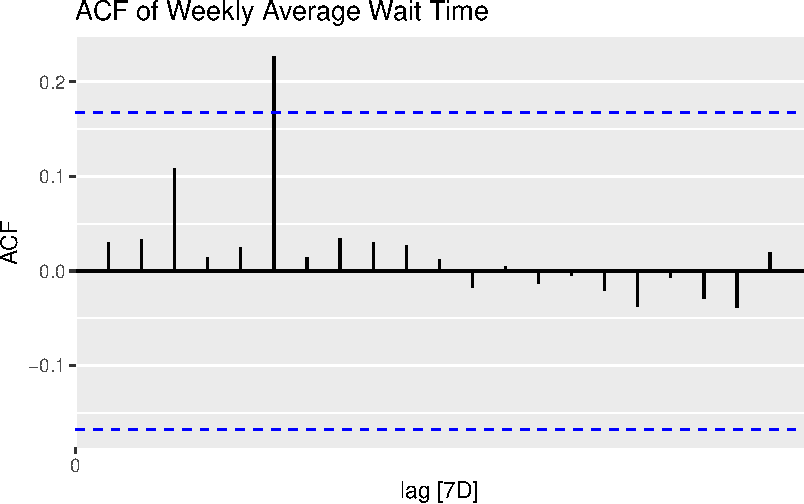
\includegraphics{final_proj_group1_files/figure-pdf/unnamed-chunk-3-2.pdf}

\begin{Shaded}
\begin{Highlighting}[]
\CommentTok{\# decomposition}
\NormalTok{decomp\_wait }\OtherTok{\textless{}{-}}\NormalTok{ df\_weekly\_wait\_ts }\SpecialCharTok{\%\textgreater{}\%}
  \FunctionTok{fill\_gaps}\NormalTok{() }\SpecialCharTok{\%\textgreater{}\%}
  \FunctionTok{mutate}\NormalTok{(}\AttributeTok{avg\_wait\_time =} \FunctionTok{if\_else}\NormalTok{(}\FunctionTok{is.na}\NormalTok{(avg\_wait\_time), }\FunctionTok{mean}\NormalTok{(avg\_wait\_time, }\AttributeTok{na.rm =} \ConstantTok{TRUE}\NormalTok{), avg\_wait\_time)) }\SpecialCharTok{\%\textgreater{}\%}
  \FunctionTok{model}\NormalTok{(}\AttributeTok{stl =} \FunctionTok{STL}\NormalTok{(avg\_wait\_time }\SpecialCharTok{\textasciitilde{}} \FunctionTok{season}\NormalTok{(}\AttributeTok{window =} \StringTok{"periodic"}\NormalTok{)))}

\CommentTok{\# extract and view decomp components}
\NormalTok{components\_wait }\OtherTok{\textless{}{-}}\NormalTok{ decomp\_wait }\SpecialCharTok{\%\textgreater{}\%}
  \FunctionTok{components}\NormalTok{()}

\CommentTok{\# plot decomp}
\NormalTok{components\_wait }\SpecialCharTok{\%\textgreater{}\%}
  \FunctionTok{autoplot}\NormalTok{() }\SpecialCharTok{+} 
  \FunctionTok{labs}\NormalTok{(}
    \AttributeTok{title =} \StringTok{"STL Decomposition of Weekly Average Wait Time"}\NormalTok{, }
    \AttributeTok{y =} \StringTok{"Average Wait Time"}\NormalTok{, }
    \AttributeTok{x =} \StringTok{"Date"}
\NormalTok{  ) }\SpecialCharTok{+}
  \FunctionTok{theme\_minimal}\NormalTok{()}
\end{Highlighting}
\end{Shaded}

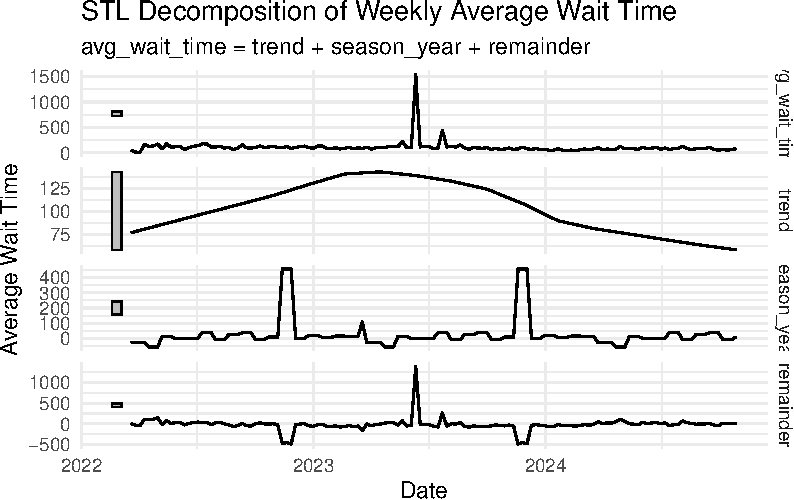
\includegraphics{final_proj_group1_files/figure-pdf/unnamed-chunk-3-3.pdf}

\paragraph{Observations}\label{observations-9}

Based on average wait time, this does not have any seasonality or cyclic
elements. Some weeks were missing data and therefore arbitrarily imputed
with the mean wait time.

\section{Data Preparation}\label{data-preparation}

Step 1: Drop all rows that are not an inbound phone call. 23, 185 rows
dropped

\begin{Shaded}
\begin{Highlighting}[]
\NormalTok{df\_phone }\OtherTok{\textless{}{-}}\NormalTok{ df }\SpecialCharTok{\%\textgreater{}\%}
  \FunctionTok{filter}\NormalTok{(CommunicationType }\SpecialCharTok{==} \StringTok{"phone"}\NormalTok{) }\SpecialCharTok{\%\textgreater{}\%}
  \FunctionTok{filter}\NormalTok{(SubCommunicationType }\SpecialCharTok{==} \StringTok{"inbound"}\NormalTok{)}
  \FunctionTok{dim}\NormalTok{(df\_phone)}
\end{Highlighting}
\end{Shaded}

\begin{verbatim}
[1] 252470      8
\end{verbatim}

Step 2: Check min/max dates. Final data should be 4/11/22 - 10/31/24 as
prior to 4/11/22 was on boarding the phone system and not representative
of operations.

\begin{Shaded}
\begin{Highlighting}[]
\NormalTok{max\_date }\OtherTok{\textless{}{-}} \FunctionTok{max}\NormalTok{(df\_phone}\SpecialCharTok{$}\NormalTok{StartTime)}
\NormalTok{min\_date }\OtherTok{\textless{}{-}} \FunctionTok{min}\NormalTok{(df\_phone}\SpecialCharTok{$}\NormalTok{StartTime)}
\FunctionTok{print}\NormalTok{(max\_date)}
\end{Highlighting}
\end{Shaded}

\begin{verbatim}
[1] "2024-10-31 23:57:27 UTC"
\end{verbatim}

\begin{Shaded}
\begin{Highlighting}[]
\FunctionTok{print}\NormalTok{(min\_date)}
\end{Highlighting}
\end{Shaded}

\begin{verbatim}
[1] "2022-03-21 16:57:05 UTC"
\end{verbatim}

\begin{Shaded}
\begin{Highlighting}[]
\NormalTok{df\_date }\OtherTok{\textless{}{-}}\NormalTok{ df\_phone }\SpecialCharTok{\%\textgreater{}\%}
  \FunctionTok{filter}\NormalTok{(StartTime }\SpecialCharTok{\textgreater{}=} \FunctionTok{as.POSIXct}\NormalTok{(}\StringTok{"2022{-}04{-}11"}\NormalTok{))}
\NormalTok{phone\_min }\OtherTok{\textless{}{-}} \FunctionTok{min}\NormalTok{(df\_date}\SpecialCharTok{$}\NormalTok{StartTime)}
\FunctionTok{print}\NormalTok{(phone\_min)}
\end{Highlighting}
\end{Shaded}

\begin{verbatim}
[1] "2022-04-11 18:28:51 UTC"
\end{verbatim}

Step 3: Separate time stamp into date, time, and day of week

\begin{Shaded}
\begin{Highlighting}[]
\NormalTok{df\_date }\OtherTok{\textless{}{-}}\NormalTok{ df\_date }\SpecialCharTok{\%\textgreater{}\%}
  \FunctionTok{mutate}\NormalTok{(}
    \AttributeTok{Date =} \FunctionTok{as.Date}\NormalTok{(StartTime),}
    \AttributeTok{Day =} \FunctionTok{weekdays}\NormalTok{(StartTime)}
\NormalTok{  )}
\end{Highlighting}
\end{Shaded}

Step 4: Drop unnecessary columns. Since this forecast is focusing on
inbound calls, we will drop the details around call length, hold times,
etc. Additionally we extracted our dates, so we will drop StartTime

\begin{Shaded}
\begin{Highlighting}[]
\NormalTok{df\_columns }\OtherTok{\textless{}{-}}\NormalTok{ df\_date }\SpecialCharTok{\%\textgreater{}\%}
  \FunctionTok{select}\NormalTok{(}\SpecialCharTok{{-}}\NormalTok{StartTime, }\SpecialCharTok{{-}}\NormalTok{EndTime, }\SpecialCharTok{{-}}\NormalTok{CommunicationType, }\SpecialCharTok{{-}}\NormalTok{SubCommunicationType, }\SpecialCharTok{{-}}\NormalTok{WaitTime, }\SpecialCharTok{{-}}\NormalTok{TimeInteracting, }\SpecialCharTok{{-}}\NormalTok{HoldTime, }\SpecialCharTok{{-}}\NormalTok{WrapUpTime)}
\end{Highlighting}
\end{Shaded}

Step 5: Add weather. Source:
\href{https://www.ncei.noaa.gov/access/search/data-search/daily-summaries?bbox=33.014,-117.462,32.418,-116.866&pageNum=1}{https://www.ncei.noaa.gov/access/search/data-search}

\begin{Shaded}
\begin{Highlighting}[]
\NormalTok{weather }\OtherTok{\textless{}{-}} \FunctionTok{read\_csv}\NormalTok{(}\FunctionTok{here}\NormalTok{(}\StringTok{"datasets/weather.csv"}\NormalTok{), }\AttributeTok{col\_types =} \FunctionTok{cols}\NormalTok{(}
   \AttributeTok{DATE =} \FunctionTok{col\_date}\NormalTok{(}\AttributeTok{format =} \StringTok{"\%Y{-}\%m{-}\%d"}\NormalTok{),  }
  \AttributeTok{TMAX =} \FunctionTok{col\_integer}\NormalTok{(),}
  \AttributeTok{TMAX\_ATTRIBUTES =} \FunctionTok{col\_character}\NormalTok{()}
\NormalTok{))}
\FunctionTok{head}\NormalTok{(weather)}
\end{Highlighting}
\end{Shaded}

\begin{verbatim}
# A tibble: 6 x 3
  DATE        TMAX TMAX_ATTRIBUTES
  <date>     <int> <chr>          
1 2024-10-31   217 W              
2 2024-10-30   222 D              
3 2024-10-29   200 W              
4 2024-10-28   217 W              
5 2024-10-27   250 W              
6 2024-10-26   233 W              
\end{verbatim}

\begin{Shaded}
\begin{Highlighting}[]
\NormalTok{weather }\OtherTok{\textless{}{-}}\NormalTok{ weather }\SpecialCharTok{\%\textgreater{}\%}
  \FunctionTok{mutate}\NormalTok{(}
    \AttributeTok{TMAX\_CEL =} \FunctionTok{as.numeric}\NormalTok{(}\FunctionTok{gsub}\NormalTok{(}\StringTok{","}\NormalTok{, }\StringTok{""}\NormalTok{, TMAX)) }\SpecialCharTok{/} \DecValTok{10}
\NormalTok{  )}
\FunctionTok{head}\NormalTok{(weather)}
\end{Highlighting}
\end{Shaded}

\begin{verbatim}
# A tibble: 6 x 4
  DATE        TMAX TMAX_ATTRIBUTES TMAX_CEL
  <date>     <int> <chr>              <dbl>
1 2024-10-31   217 W                   21.7
2 2024-10-30   222 D                   22.2
3 2024-10-29   200 W                   20  
4 2024-10-28   217 W                   21.7
5 2024-10-27   250 W                   25  
6 2024-10-26   233 W                   23.3
\end{verbatim}

\begin{Shaded}
\begin{Highlighting}[]
\NormalTok{df\_weather }\OtherTok{\textless{}{-}}\NormalTok{ df\_columns }\SpecialCharTok{\%\textgreater{}\%}
  \FunctionTok{left\_join}\NormalTok{(weather }\SpecialCharTok{\%\textgreater{}\%} \FunctionTok{select}\NormalTok{(DATE, TMAX\_CEL), }\AttributeTok{by =} \FunctionTok{c}\NormalTok{(}\StringTok{"Date"} \OtherTok{=} \StringTok{"DATE"}\NormalTok{))}
\end{Highlighting}
\end{Shaded}

\begin{Shaded}
\begin{Highlighting}[]
\NormalTok{na\_count }\OtherTok{\textless{}{-}} \FunctionTok{sapply}\NormalTok{(df\_weather, }\ControlFlowTok{function}\NormalTok{(x) }\FunctionTok{sum}\NormalTok{(}\FunctionTok{is.na}\NormalTok{(x)))}
\FunctionTok{print}\NormalTok{(na\_count)}
\end{Highlighting}
\end{Shaded}

\begin{verbatim}
    Date      Day TMAX_CEL 
       0        0        0 
\end{verbatim}

Step 6: Sum up by day

\begin{Shaded}
\begin{Highlighting}[]
\NormalTok{df\_prepped }\OtherTok{\textless{}{-}}\NormalTok{ df\_weather }\SpecialCharTok{\%\textgreater{}\%}
  \FunctionTok{group\_by}\NormalTok{(Date, Day, TMAX\_CEL) }\SpecialCharTok{\%\textgreater{}\%}
  \FunctionTok{summarise}\NormalTok{(}\AttributeTok{total\_calls =} \FunctionTok{n}\NormalTok{(), }\AttributeTok{.groups =} \StringTok{"drop"}\NormalTok{)}
\end{Highlighting}
\end{Shaded}

\begin{Shaded}
\begin{Highlighting}[]
\FunctionTok{write\_csv}\NormalTok{(df\_prepped, }\FunctionTok{here}\NormalTok{(}\StringTok{"datasets/calls\_prepped.csv"}\NormalTok{))}
\end{Highlighting}
\end{Shaded}

\section{New Data Exploration}\label{new-data-exploration}

\begin{Shaded}
\begin{Highlighting}[]
\FunctionTok{library}\NormalTok{(gridExtra)}
\end{Highlighting}
\end{Shaded}

\begin{verbatim}

Attaching package: 'gridExtra'
\end{verbatim}

\begin{verbatim}
The following object is masked from 'package:dplyr':

    combine
\end{verbatim}

\begin{Shaded}
\begin{Highlighting}[]
\NormalTok{temp\_scatter }\OtherTok{\textless{}{-}}\NormalTok{ df\_prepped}\SpecialCharTok{|\textgreater{}}
  \FunctionTok{ggplot}\NormalTok{(}\FunctionTok{aes}\NormalTok{(}\AttributeTok{x =}\NormalTok{ total\_calls, }\AttributeTok{y =}\NormalTok{TMAX\_CEL)) }\SpecialCharTok{+} 
  \FunctionTok{geom\_point}\NormalTok{() }\SpecialCharTok{+} 
  \FunctionTok{theme\_minimal}\NormalTok{() }\SpecialCharTok{+} 
  \FunctionTok{labs}\NormalTok{(}\AttributeTok{title =} \StringTok{"Scatter plot, Temperature and Call Volume"}\NormalTok{)}\SpecialCharTok{+} 
  \FunctionTok{geom\_smooth}\NormalTok{(}\AttributeTok{method =}\NormalTok{ lm)}

\NormalTok{day\_box }\OtherTok{\textless{}{-}}\NormalTok{ df\_prepped}\SpecialCharTok{|\textgreater{}}
  \FunctionTok{ggplot}\NormalTok{(}\FunctionTok{aes}\NormalTok{(}\AttributeTok{x =}\NormalTok{ Day, }\AttributeTok{y =}\NormalTok{ total\_calls)) }\SpecialCharTok{+}
  \FunctionTok{geom\_boxplot}\NormalTok{(}\AttributeTok{fill =} \StringTok{"lightblue"}\NormalTok{, }\AttributeTok{color =} \StringTok{"darkblue"}\NormalTok{) }\SpecialCharTok{+}
  \FunctionTok{labs}\NormalTok{(}\AttributeTok{title =} \StringTok{"Total Calls by Day of the Week"}\NormalTok{, }\AttributeTok{x =} \StringTok{"Day of the Week"}\NormalTok{, }\AttributeTok{y =} \StringTok{"Total Calls"}\NormalTok{) }\SpecialCharTok{+}
  \FunctionTok{theme\_minimal}\NormalTok{()}\SpecialCharTok{+} 
  \FunctionTok{theme}\NormalTok{(}\AttributeTok{axis.text.x =} \FunctionTok{element\_text}\NormalTok{(}\AttributeTok{angle =} \DecValTok{45}\NormalTok{, }\AttributeTok{hjust =} \DecValTok{1}\NormalTok{))}

\FunctionTok{grid.arrange}\NormalTok{(temp\_scatter, day\_box, }\AttributeTok{ncol =} \DecValTok{2}\NormalTok{) }
\end{Highlighting}
\end{Shaded}

\begin{verbatim}
`geom_smooth()` using formula = 'y ~ x'
\end{verbatim}

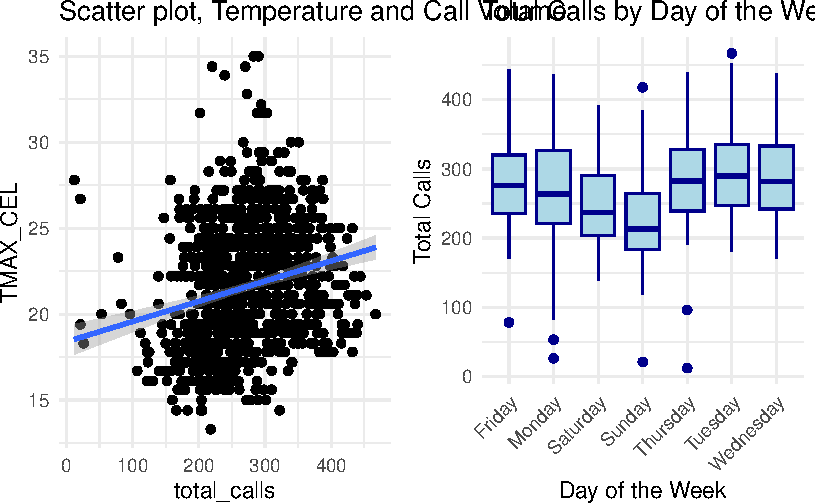
\includegraphics{final_proj_group1_files/figure-pdf/scatter_plots-1.pdf}

\section{Modeling}\label{modeling}

\begin{Shaded}
\begin{Highlighting}[]
\CommentTok{\# make a modeling df from the prepped df for redundancy purposes}
\NormalTok{model\_df }\OtherTok{\textless{}{-}}\NormalTok{ df\_prepped}
\CommentTok{\#class(model\_df$Date)}

\CommentTok{\# convert df to tsibble}
\NormalTok{model\_ts }\OtherTok{\textless{}{-}}\NormalTok{ model\_df }\SpecialCharTok{|\textgreater{}}
  \FunctionTok{as\_tsibble}\NormalTok{(}\AttributeTok{index =}\NormalTok{ Date)}

\CommentTok{\#head(model\_df)}
\end{Highlighting}
\end{Shaded}

\subsection{Data Partitioning}\label{data-partitioning}

\begin{Shaded}
\begin{Highlighting}[]
\CommentTok{\# Partition the dataset into training and validation set}
\CommentTok{\# Forecast horizon is 30 days, meaning validation = 30 days}

\CommentTok{\# set split date}
\NormalTok{split\_date }\OtherTok{\textless{}{-}} \FunctionTok{as.Date}\NormalTok{(}\StringTok{"2024{-}10{-}01"}\NormalTok{)}

\NormalTok{tng\_df }\OtherTok{\textless{}{-}}\NormalTok{ model\_ts }\SpecialCharTok{|\textgreater{}}
  \FunctionTok{filter}\NormalTok{(Date }\SpecialCharTok{\textless{}}\NormalTok{ split\_date)}

\CommentTok{\#head(tng\_df, 5)}
\CommentTok{\#tail(tng\_df, 5)}

\NormalTok{validation\_df }\OtherTok{\textless{}{-}}\NormalTok{ model\_ts }\SpecialCharTok{|\textgreater{}}
  \FunctionTok{filter}\NormalTok{(Date }\SpecialCharTok{\textgreater{}=}\NormalTok{ split\_date)}

\CommentTok{\#head(validation\_df, 5)}
\CommentTok{\#tail(validation\_df, 5)}
\end{Highlighting}
\end{Shaded}

\begin{Shaded}
\begin{Highlighting}[]
\CommentTok{\# initialize empty performance metrics tibble to store results}
\NormalTok{performance\_metrics }\OtherTok{\textless{}{-}} \FunctionTok{tibble}\NormalTok{(}
  \AttributeTok{Model =} \FunctionTok{character}\NormalTok{(),}
  \AttributeTok{RMSE =} \FunctionTok{numeric}\NormalTok{(),}
  \AttributeTok{MAE =} \FunctionTok{numeric}\NormalTok{(),}
  \AttributeTok{MAPE =} \FunctionTok{numeric}\NormalTok{()}
\NormalTok{)}
\end{Highlighting}
\end{Shaded}

\subsubsection{Seasonal Naive}\label{seasonal-naive}

\begin{Shaded}
\begin{Highlighting}[]
\CommentTok{\# fit the model to training data}
\NormalTok{snaive\_model }\OtherTok{\textless{}{-}}\NormalTok{ tng\_df }\SpecialCharTok{|\textgreater{}}
  \FunctionTok{model}\NormalTok{(}\FunctionTok{SNAIVE}\NormalTok{(total\_calls }\SpecialCharTok{\textasciitilde{}} \FunctionTok{lag}\NormalTok{(}\DecValTok{7}\NormalTok{)))}

\CommentTok{\# forecast validation period}
\NormalTok{snaive\_forecast }\OtherTok{\textless{}{-}}\NormalTok{ snaive\_model }\SpecialCharTok{|\textgreater{}}
  \FunctionTok{forecast}\NormalTok{(}\AttributeTok{h =} \FunctionTok{nrow}\NormalTok{(validation\_df))}

\CommentTok{\# performance metrics}
\NormalTok{snaive\_performance }\OtherTok{\textless{}{-}}\NormalTok{ snaive\_forecast }\SpecialCharTok{|\textgreater{}}
  \FunctionTok{accuracy}\NormalTok{(}\AttributeTok{data =}\NormalTok{ validation\_df)}

\CommentTok{\# add results to performance metrics table}
\NormalTok{performance\_metrics }\OtherTok{\textless{}{-}}\NormalTok{ performance\_metrics }\SpecialCharTok{|\textgreater{}}
  \FunctionTok{add\_row}\NormalTok{(}\AttributeTok{Model =} \StringTok{"SNAIVE"}\NormalTok{,}
          \AttributeTok{RMSE =}\NormalTok{ snaive\_performance}\SpecialCharTok{$}\NormalTok{RMSE,}
          \AttributeTok{MAE =}\NormalTok{ snaive\_performance}\SpecialCharTok{$}\NormalTok{MAE,}
          \AttributeTok{MAPE =}\NormalTok{ snaive\_performance}\SpecialCharTok{$}\NormalTok{MAPE}
\NormalTok{          )}
\CommentTok{\# view table}
\NormalTok{performance\_metrics}
\end{Highlighting}
\end{Shaded}

\begin{verbatim}
# A tibble: 1 x 4
  Model   RMSE   MAE  MAPE
  <chr>  <dbl> <dbl> <dbl>
1 SNAIVE  21.8  17.2  8.59
\end{verbatim}

\begin{Shaded}
\begin{Highlighting}[]
\CommentTok{\# Visualize}
\NormalTok{snaive\_plot }\OtherTok{\textless{}{-}} \FunctionTok{autoplot}\NormalTok{(snaive\_forecast, tng\_df) }\SpecialCharTok{+} 
  \FunctionTok{autolayer}\NormalTok{(validation\_df, total\_calls) }\SpecialCharTok{+} 
  \FunctionTok{autolayer}\NormalTok{(snaive\_forecast, }\AttributeTok{color =} \StringTok{"red"}\NormalTok{, }\AttributeTok{alpha =} \FloatTok{0.25}\NormalTok{) }\SpecialCharTok{+}
  \FunctionTok{ggtitle}\NormalTok{(}\StringTok{"SNAIVE Forecast v. Validation Data"}\NormalTok{) }\SpecialCharTok{+} 
  \FunctionTok{labs}\NormalTok{(}\AttributeTok{y =} \StringTok{"Total Calls"}\NormalTok{)}
\end{Highlighting}
\end{Shaded}

\begin{verbatim}
Scale for fill_ramp is already present.
Adding another scale for fill_ramp, which will replace the existing scale.
\end{verbatim}

\begin{Shaded}
\begin{Highlighting}[]
\NormalTok{snaive\_plot}
\end{Highlighting}
\end{Shaded}

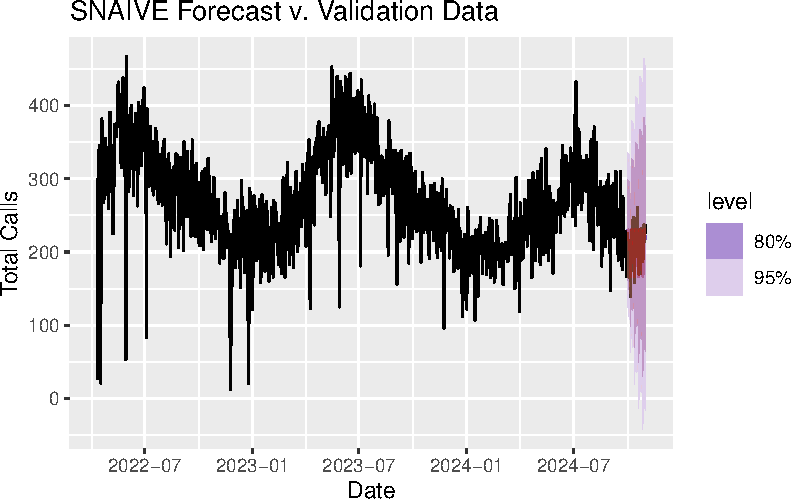
\includegraphics{final_proj_group1_files/figure-pdf/unnamed-chunk-8-1.pdf}

\subsubsection{Auto ARIMA (non-seasonal)}\label{auto-arima-non-seasonal}

\begin{Shaded}
\begin{Highlighting}[]
\CommentTok{\# fit the model to the training data}
\NormalTok{auto\_ARIMA }\OtherTok{\textless{}{-}}\NormalTok{ tng\_df }\SpecialCharTok{|\textgreater{}}
  \FunctionTok{model}\NormalTok{(}\FunctionTok{ARIMA}\NormalTok{(total\_calls }\SpecialCharTok{\textasciitilde{}} \FunctionTok{PDQ}\NormalTok{(}\DecValTok{0}\NormalTok{,}\DecValTok{0}\NormalTok{,}\DecValTok{0}\NormalTok{)) }\CommentTok{\# 0 indicates no seasonal terms}
\NormalTok{        )}

\CommentTok{\# view the auto selected model parameters}
\FunctionTok{report}\NormalTok{(auto\_ARIMA)}
\end{Highlighting}
\end{Shaded}

\begin{verbatim}
Series: total_calls 
Model: ARIMA(5,1,1) 

Coefficients:
          ar1      ar2      ar3      ar4      ar5      ma1
      -0.1718  -0.3504  -0.3171  -0.3087  -0.3303  -0.5390
s.e.   0.0522   0.0383   0.0378   0.0356   0.0379   0.0505

sigma^2 estimated as 1970:  log likelihood=-4704.34
AIC=9422.69   AICc=9422.81   BIC=9456.33
\end{verbatim}

\begin{Shaded}
\begin{Highlighting}[]
\CommentTok{\# forecast the validation period}
\NormalTok{auto\_ARIMA\_forecast }\OtherTok{\textless{}{-}}\NormalTok{ auto\_ARIMA }\SpecialCharTok{|\textgreater{}}
  \FunctionTok{forecast}\NormalTok{(}\AttributeTok{h =} \FunctionTok{nrow}\NormalTok{(validation\_df))}

\CommentTok{\# performance metrics}
\NormalTok{AA\_perf\_metrics }\OtherTok{\textless{}{-}}\NormalTok{ auto\_ARIMA\_forecast }\SpecialCharTok{|\textgreater{}} 
  \FunctionTok{accuracy}\NormalTok{(}\AttributeTok{data =}\NormalTok{ validation\_df)}

\CommentTok{\# add performance metrics to table}
\NormalTok{performance\_metrics }\OtherTok{\textless{}{-}}\NormalTok{ performance\_metrics }\SpecialCharTok{|\textgreater{}} 
  \FunctionTok{add\_row}\NormalTok{(}\AttributeTok{Model =} \StringTok{"Auto Arima"}\NormalTok{,}
          \AttributeTok{RMSE =}\NormalTok{ AA\_perf\_metrics}\SpecialCharTok{$}\NormalTok{RMSE,}
          \AttributeTok{MAE =}\NormalTok{ AA\_perf\_metrics}\SpecialCharTok{$}\NormalTok{MAE,}
          \AttributeTok{MAPE =}\NormalTok{ AA\_perf\_metrics}\SpecialCharTok{$}\NormalTok{MAPE}
\NormalTok{          )}

\CommentTok{\# view metrics}
\NormalTok{performance\_metrics}
\end{Highlighting}
\end{Shaded}

\begin{verbatim}
# A tibble: 2 x 4
  Model       RMSE   MAE  MAPE
  <chr>      <dbl> <dbl> <dbl>
1 SNAIVE      21.8  17.2  8.59
2 Auto Arima  26.1  21.2 10.8 
\end{verbatim}

\begin{Shaded}
\begin{Highlighting}[]
\CommentTok{\# Visualize}
\NormalTok{AA\_plot }\OtherTok{\textless{}{-}} \FunctionTok{autoplot}\NormalTok{(auto\_ARIMA\_forecast, tng\_df) }\SpecialCharTok{+} 
  \FunctionTok{autolayer}\NormalTok{(validation\_df, total\_calls) }\SpecialCharTok{+} 
  \FunctionTok{autolayer}\NormalTok{(auto\_ARIMA\_forecast, }\AttributeTok{color =} \StringTok{"red"}\NormalTok{, }\AttributeTok{alpha =} \FloatTok{0.25}\NormalTok{) }\SpecialCharTok{+}
  \FunctionTok{ggtitle}\NormalTok{(}\StringTok{"Auto ARIMA(5,1,1) v. Validation Data"}\NormalTok{) }\SpecialCharTok{+} 
  \FunctionTok{labs}\NormalTok{(}\AttributeTok{y =} \StringTok{"Total Calls"}\NormalTok{)}
\end{Highlighting}
\end{Shaded}

\begin{verbatim}
Scale for fill_ramp is already present.
Adding another scale for fill_ramp, which will replace the existing scale.
\end{verbatim}

\begin{Shaded}
\begin{Highlighting}[]
\NormalTok{AA\_plot}
\end{Highlighting}
\end{Shaded}

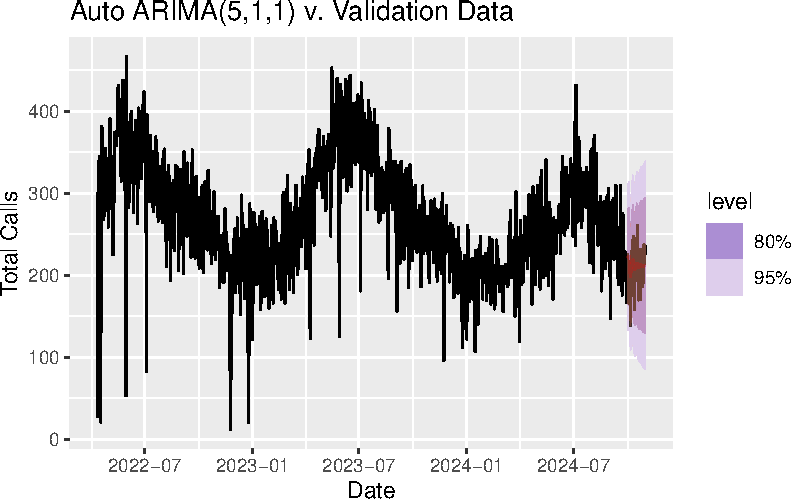
\includegraphics{final_proj_group1_files/figure-pdf/unnamed-chunk-11-1.pdf}

\subsubsection{Seasonal Auto ARIMA}\label{seasonal-auto-arima}

\begin{Shaded}
\begin{Highlighting}[]
\CommentTok{\# fit the model to the training data}
\NormalTok{SAA\_Model }\OtherTok{\textless{}{-}}\NormalTok{ tng\_df }\SpecialCharTok{|\textgreater{}}
  \FunctionTok{model}\NormalTok{(}\FunctionTok{ARIMA}\NormalTok{(total\_calls))}

\CommentTok{\# view the auto selected model parameters}
\FunctionTok{report}\NormalTok{(SAA\_Model)}
\end{Highlighting}
\end{Shaded}

\begin{verbatim}
Series: total_calls 
Model: ARIMA(1,1,2)(2,0,0)[7] 

Coefficients:
         ar1      ma1      ma2    sar1    sar2
      0.1006  -0.8684  -0.0578  0.2702  0.2144
s.e.  0.2050   0.2066   0.1877  0.0352  0.0348

sigma^2 estimated as 1932:  log likelihood=-4696.29
AIC=9404.58   AICc=9404.68   BIC=9433.42
\end{verbatim}

\begin{Shaded}
\begin{Highlighting}[]
\CommentTok{\# forecast the validation period}
\NormalTok{SAA\_forecast }\OtherTok{\textless{}{-}}\NormalTok{ SAA\_Model }\SpecialCharTok{|\textgreater{}}
  \FunctionTok{forecast}\NormalTok{(}\AttributeTok{h =} \FunctionTok{nrow}\NormalTok{(validation\_df))}

\CommentTok{\# performance metrics}
\NormalTok{SAA\_perf\_metrics }\OtherTok{\textless{}{-}}\NormalTok{ SAA\_forecast }\SpecialCharTok{|\textgreater{}} 
  \FunctionTok{accuracy}\NormalTok{(}\AttributeTok{data =}\NormalTok{ validation\_df)}

\CommentTok{\# add performance metrics to table}
\NormalTok{performance\_metrics }\OtherTok{\textless{}{-}}\NormalTok{ performance\_metrics }\SpecialCharTok{|\textgreater{}} 
  \FunctionTok{add\_row}\NormalTok{(}\AttributeTok{Model =} \StringTok{"Seasonal Auto Arima"}\NormalTok{,}
          \AttributeTok{RMSE =}\NormalTok{ SAA\_perf\_metrics}\SpecialCharTok{$}\NormalTok{RMSE,}
          \AttributeTok{MAE =}\NormalTok{ SAA\_perf\_metrics}\SpecialCharTok{$}\NormalTok{MAE,}
          \AttributeTok{MAPE =}\NormalTok{ SAA\_perf\_metrics}\SpecialCharTok{$}\NormalTok{MAPE}
\NormalTok{          )}

\CommentTok{\# view metrics}
\NormalTok{performance\_metrics}
\end{Highlighting}
\end{Shaded}

\begin{verbatim}
# A tibble: 3 x 4
  Model                RMSE   MAE  MAPE
  <chr>               <dbl> <dbl> <dbl>
1 SNAIVE               21.8  17.2  8.59
2 Auto Arima           26.1  21.2 10.8 
3 Seasonal Auto Arima  25.3  20.8 10.7 
\end{verbatim}

\begin{Shaded}
\begin{Highlighting}[]
\CommentTok{\# visualize}
\NormalTok{SAA\_plot }\OtherTok{\textless{}{-}} \FunctionTok{autoplot}\NormalTok{(SAA\_forecast, tng\_df) }\SpecialCharTok{+} 
  \FunctionTok{autolayer}\NormalTok{(validation\_df, total\_calls) }\SpecialCharTok{+} 
  \FunctionTok{autolayer}\NormalTok{(SAA\_forecast, }\AttributeTok{color =} \StringTok{"red"}\NormalTok{, }\AttributeTok{alpha =} \FloatTok{0.25}\NormalTok{) }\SpecialCharTok{+}
  \FunctionTok{ggtitle}\NormalTok{(}\StringTok{"Seasonal Auto Arima(1,1,2)(2,0,0)[7] v. Validation Data"}\NormalTok{) }\SpecialCharTok{+} 
  \FunctionTok{labs}\NormalTok{(}\AttributeTok{y =} \StringTok{"Total Calls"}\NormalTok{)}
\end{Highlighting}
\end{Shaded}

\begin{verbatim}
Scale for fill_ramp is already present.
Adding another scale for fill_ramp, which will replace the existing scale.
\end{verbatim}

\begin{Shaded}
\begin{Highlighting}[]
\NormalTok{SAA\_plot}
\end{Highlighting}
\end{Shaded}

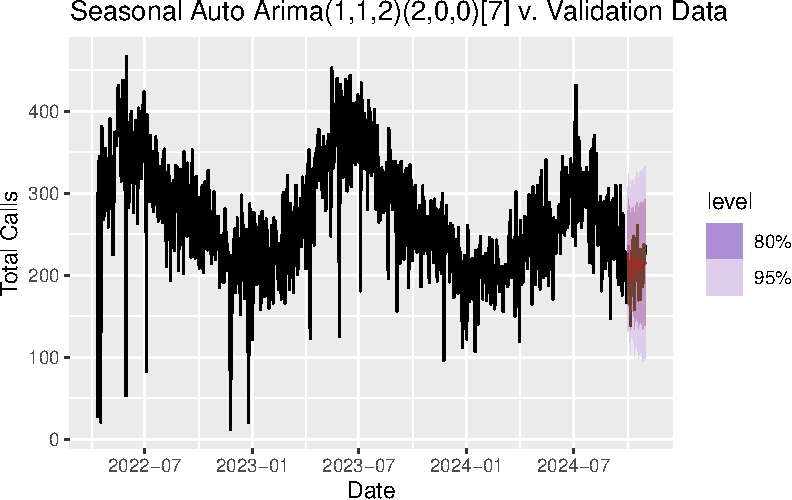
\includegraphics{final_proj_group1_files/figure-pdf/unnamed-chunk-14-1.pdf}

\subsubsection{Auto ARIMA (w/ Max Temp)}\label{auto-arima-w-max-temp}

\begin{Shaded}
\begin{Highlighting}[]
\CommentTok{\# fit the model to the training data}
\NormalTok{AA\_temp\_model }\OtherTok{\textless{}{-}}\NormalTok{ tng\_df }\SpecialCharTok{|\textgreater{}}
  \FunctionTok{model}\NormalTok{(}\FunctionTok{ARIMA}\NormalTok{(total\_calls }\SpecialCharTok{\textasciitilde{}} \FunctionTok{PDQ}\NormalTok{(}\DecValTok{0}\NormalTok{,}\DecValTok{0}\NormalTok{,}\DecValTok{0}\NormalTok{) }\SpecialCharTok{+} 
\NormalTok{                TMAX\_CEL))}

\CommentTok{\# view the auto selected model parameters}
\FunctionTok{report}\NormalTok{(AA\_temp\_model)}
\end{Highlighting}
\end{Shaded}

\begin{verbatim}
Series: total_calls 
Model: LM w/ ARIMA(1,1,5) errors 

Coefficients:
         ar1      ma1      ma2     ma3     ma4     ma5  TMAX_CEL
      0.3317  -1.0353  -0.0261  0.0552  0.0355  0.0621    1.1867
s.e.  0.1391   0.1380   0.1145  0.0527  0.0653  0.0432    0.7413

sigma^2 estimated as 2145:  log likelihood=-4742.06
AIC=9500.12   AICc=9500.28   BIC=9538.56
\end{verbatim}

\begin{Shaded}
\begin{Highlighting}[]
\CommentTok{\# forecast the validation period}
\NormalTok{AA\_temp\_forecast }\OtherTok{\textless{}{-}}\NormalTok{ AA\_temp\_model }\SpecialCharTok{|\textgreater{}}
  \FunctionTok{forecast}\NormalTok{(}\AttributeTok{new\_data =}\NormalTok{ validation\_df)}

\CommentTok{\# performance metrics}
\NormalTok{AA\_temp\_perf\_metrics }\OtherTok{\textless{}{-}}\NormalTok{ AA\_temp\_forecast }\SpecialCharTok{|\textgreater{}} 
  \FunctionTok{accuracy}\NormalTok{(}\AttributeTok{data =}\NormalTok{ validation\_df)}

\CommentTok{\# add performance metrics to table}
\NormalTok{performance\_metrics }\OtherTok{\textless{}{-}}\NormalTok{ performance\_metrics }\SpecialCharTok{|\textgreater{}} 
  \FunctionTok{add\_row}\NormalTok{(}\AttributeTok{Model =} \StringTok{"Auto Arima (w/ Temp)"}\NormalTok{,}
          \AttributeTok{RMSE =}\NormalTok{ AA\_temp\_perf\_metrics}\SpecialCharTok{$}\NormalTok{RMSE,}
          \AttributeTok{MAE =}\NormalTok{ AA\_temp\_perf\_metrics}\SpecialCharTok{$}\NormalTok{MAE,}
          \AttributeTok{MAPE =}\NormalTok{ AA\_temp\_perf\_metrics}\SpecialCharTok{$}\NormalTok{MAPE}
\NormalTok{          )}

\CommentTok{\# view metrics}
\NormalTok{performance\_metrics}
\end{Highlighting}
\end{Shaded}

\begin{verbatim}
# A tibble: 4 x 4
  Model                 RMSE   MAE  MAPE
  <chr>                <dbl> <dbl> <dbl>
1 SNAIVE                21.8  17.2  8.59
2 Auto Arima            26.1  21.2 10.8 
3 Seasonal Auto Arima   25.3  20.8 10.7 
4 Auto Arima (w/ Temp)  30.1  23.9 12.5 
\end{verbatim}

\begin{Shaded}
\begin{Highlighting}[]
\CommentTok{\# visualize}
\NormalTok{AA\_temp\_plot }\OtherTok{\textless{}{-}} \FunctionTok{autoplot}\NormalTok{(AA\_temp\_forecast, tng\_df) }\SpecialCharTok{+} 
  \FunctionTok{autolayer}\NormalTok{(validation\_df, total\_calls) }\SpecialCharTok{+} 
  \FunctionTok{autolayer}\NormalTok{(AA\_temp\_forecast, }\AttributeTok{color =} \StringTok{"red"}\NormalTok{, }\AttributeTok{alpha =} \FloatTok{0.25}\NormalTok{) }\SpecialCharTok{+}
  \FunctionTok{ggtitle}\NormalTok{(}\StringTok{"Auto Arima w/ Max Temp v. Validation Data"}\NormalTok{) }\SpecialCharTok{+} 
  \FunctionTok{labs}\NormalTok{(}\AttributeTok{y =} \StringTok{"Total Calls"}\NormalTok{)}
\end{Highlighting}
\end{Shaded}

\begin{verbatim}
Scale for fill_ramp is already present.
Adding another scale for fill_ramp, which will replace the existing scale.
\end{verbatim}

\subsubsection{Seasonal Auto ARIMA (w/ Max
Temp)}\label{seasonal-auto-arima-w-max-temp}

\begin{Shaded}
\begin{Highlighting}[]
\CommentTok{\# fit the model to the training data}
\NormalTok{SAA\_temp\_model }\OtherTok{\textless{}{-}}\NormalTok{ tng\_df }\SpecialCharTok{|\textgreater{}}
  \FunctionTok{model}\NormalTok{(}\FunctionTok{ARIMA}\NormalTok{(total\_calls }\SpecialCharTok{\textasciitilde{}}\NormalTok{ TMAX\_CEL))}

\CommentTok{\# view the auto selected model parameters}
\FunctionTok{report}\NormalTok{(SAA\_temp\_model)}
\end{Highlighting}
\end{Shaded}

\begin{verbatim}
Series: total_calls 
Model: LM w/ ARIMA(1,1,2)(2,0,0)[7] errors 

Coefficients:
         ar1      ma1      ma2    sar1    sar2  TMAX_CEL
      0.0863  -0.8578  -0.0688  0.2702  0.2149    1.1083
s.e.  0.2063   0.2071   0.1886  0.0352  0.0348    0.6777

sigma^2 estimated as 1928:  log likelihood=-4694.96
AIC=9403.93   AICc=9404.05   BIC=9437.57
\end{verbatim}

\begin{Shaded}
\begin{Highlighting}[]
\CommentTok{\# forecast the validation period}
\NormalTok{SAA\_temp\_forecast }\OtherTok{\textless{}{-}}\NormalTok{ SAA\_temp\_model }\SpecialCharTok{|\textgreater{}}
  \FunctionTok{forecast}\NormalTok{(}\AttributeTok{new\_data =}\NormalTok{ validation\_df)}

\CommentTok{\# performance metrics}
\NormalTok{SAA\_temp\_perf\_metrics }\OtherTok{\textless{}{-}}\NormalTok{ SAA\_temp\_forecast }\SpecialCharTok{|\textgreater{}} 
  \FunctionTok{accuracy}\NormalTok{(}\AttributeTok{data =}\NormalTok{ validation\_df)}

\CommentTok{\# add performance metrics to table}
\NormalTok{performance\_metrics }\OtherTok{\textless{}{-}}\NormalTok{ performance\_metrics }\SpecialCharTok{|\textgreater{}} 
  \FunctionTok{add\_row}\NormalTok{(}\AttributeTok{Model =} \StringTok{"Seasonal Auto Arima (w/ Temp)"}\NormalTok{,}
          \AttributeTok{RMSE =}\NormalTok{ SAA\_temp\_perf\_metrics}\SpecialCharTok{$}\NormalTok{RMSE,}
          \AttributeTok{MAE =}\NormalTok{ SAA\_temp\_perf\_metrics}\SpecialCharTok{$}\NormalTok{MAE,}
          \AttributeTok{MAPE =}\NormalTok{ SAA\_temp\_perf\_metrics}\SpecialCharTok{$}\NormalTok{MAPE}
\NormalTok{          )}

\CommentTok{\# view metrics}
\NormalTok{performance\_metrics}
\end{Highlighting}
\end{Shaded}

\begin{verbatim}
# A tibble: 5 x 4
  Model                          RMSE   MAE  MAPE
  <chr>                         <dbl> <dbl> <dbl>
1 SNAIVE                         21.8  17.2  8.59
2 Auto Arima                     26.1  21.2 10.8 
3 Seasonal Auto Arima            25.3  20.8 10.7 
4 Auto Arima (w/ Temp)           30.1  23.9 12.5 
5 Seasonal Auto Arima (w/ Temp)  26.3  21.8 11.1 
\end{verbatim}

\begin{Shaded}
\begin{Highlighting}[]
\CommentTok{\# visualize}
\NormalTok{SAA\_temp\_plot }\OtherTok{\textless{}{-}} \FunctionTok{autoplot}\NormalTok{(SAA\_temp\_forecast, tng\_df) }\SpecialCharTok{+} 
  \FunctionTok{autolayer}\NormalTok{(validation\_df, total\_calls) }\SpecialCharTok{+} 
  \FunctionTok{autolayer}\NormalTok{(SAA\_temp\_forecast, }\AttributeTok{color =} \StringTok{"red"}\NormalTok{, }\AttributeTok{alpha =} \FloatTok{0.25}\NormalTok{) }\SpecialCharTok{+}
  \FunctionTok{ggtitle}\NormalTok{(}\StringTok{"Seasonal Auto Arima w/ Max Temp v. Validation Data"}\NormalTok{) }\SpecialCharTok{+} 
  \FunctionTok{labs}\NormalTok{(}\AttributeTok{y =} \StringTok{"Total Calls"}\NormalTok{)}
\end{Highlighting}
\end{Shaded}

\begin{verbatim}
Scale for fill_ramp is already present.
Adding another scale for fill_ramp, which will replace the existing scale.
\end{verbatim}

\subsection{Model Selection}\label{model-selection}

Upon examination of the performance metrics for the selected models it
was found that the model with the best performance metrics was the
Seasonal Auto ARIMA model which selected parameters of pdq(5,0,0)
PDQ(1,0,0) with a period set to 7 days. The model had RMSE = 30.8575 and
MAE = 25.3675. These values edge out the Seasonal Auto ARIMA model that
includes the max temperature for the day by a small amount with the
exception of the performance metric MAPE, which outperformed the SAA
model with no temperature 93.8061 compared to 94.1282. Both models
performed well, however the model that did not include the maximum
temperature for the day has been selected as the model with the highest
performance metrics.

\subsubsection{SNAIVE Model Applied to Entire
Series}\label{snaive-model-applied-to-entire-series}

\begin{Shaded}
\begin{Highlighting}[]
\CommentTok{\# refit pre{-}trained SNAIVE model to entire dataset}
\NormalTok{SNAIVE\_refit }\OtherTok{\textless{}{-}}\NormalTok{ snaive\_model }\SpecialCharTok{|\textgreater{}}
  \FunctionTok{refit}\NormalTok{(model\_ts)}

\CommentTok{\# forecast the next 31 days}
\NormalTok{SNAIVE\_final\_forecast }\OtherTok{\textless{}{-}}\NormalTok{ SNAIVE\_refit }\SpecialCharTok{|\textgreater{}}
  \FunctionTok{forecast}\NormalTok{(}\AttributeTok{h =} \DecValTok{31}\NormalTok{)}

\CommentTok{\# Visualize the forecast}
\NormalTok{SNAIVE\_final\_plot }\OtherTok{\textless{}{-}} \FunctionTok{autoplot}\NormalTok{(SNAIVE\_final\_forecast, model\_ts) }\SpecialCharTok{+}
  \FunctionTok{ggtitle}\NormalTok{(}\StringTok{"31{-}Day Forecast using Refitted SNAIVE Model"}\NormalTok{) }\SpecialCharTok{+}
  \FunctionTok{labs}\NormalTok{(}\AttributeTok{y =} \StringTok{"Total Calls"}\NormalTok{, }\AttributeTok{x =} \StringTok{"Date"}\NormalTok{)}

\CommentTok{\# display the plot}
\NormalTok{SNAIVE\_final\_plot}
\end{Highlighting}
\end{Shaded}

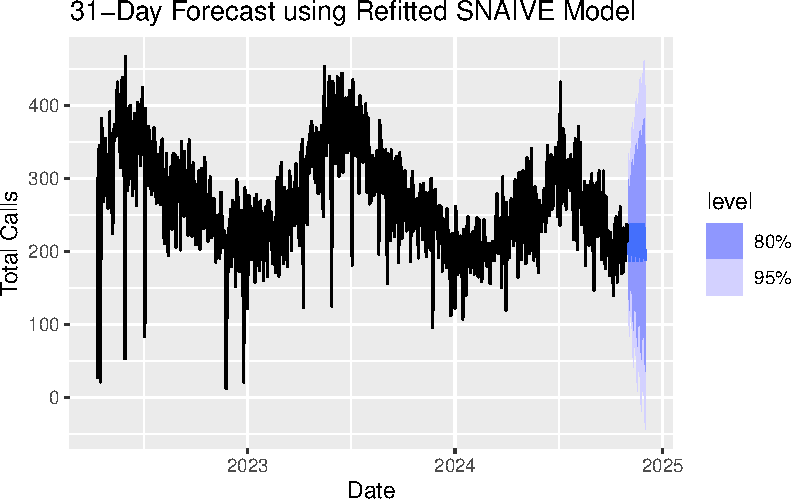
\includegraphics{final_proj_group1_files/figure-pdf/unnamed-chunk-21-1.pdf}

\begin{Shaded}
\begin{Highlighting}[]
\CommentTok{\# get November actual values into a df}
\NormalTok{nov\_df }\OtherTok{\textless{}{-}} \FunctionTok{read.csv}\NormalTok{(}\FunctionTok{here}\NormalTok{(}\StringTok{"datasets/Nov\_edify\_calls.csv"}\NormalTok{))}

\CommentTok{\# clean so it is just inbound phone calls}
\NormalTok{nov\_clean }\OtherTok{\textless{}{-}}\NormalTok{ nov\_df }\SpecialCharTok{|\textgreater{}} 
  \FunctionTok{filter}\NormalTok{(Communication.Type }\SpecialCharTok{==} \StringTok{"phone"}\NormalTok{) }\SpecialCharTok{\%\textgreater{}\%}
  \FunctionTok{filter}\NormalTok{(Sub.Communication.Type }\SpecialCharTok{==} \StringTok{"inbound"}\NormalTok{)}

\CommentTok{\# drop End.Time, Communication.Type, Sub.Communication.Type}
\NormalTok{nov\_clean }\OtherTok{\textless{}{-}}\NormalTok{ nov\_clean }\SpecialCharTok{|\textgreater{}} 
  \FunctionTok{select}\NormalTok{(}\SpecialCharTok{{-}}\NormalTok{End.Time, }\SpecialCharTok{{-}}\NormalTok{Communication.Type, }\SpecialCharTok{{-}}\NormalTok{Sub.Communication.Type)}

\CommentTok{\# get Start.time to just date format}
\NormalTok{nov\_clean }\OtherTok{\textless{}{-}}\NormalTok{ nov\_clean }\SpecialCharTok{|\textgreater{}}
  \FunctionTok{mutate}\NormalTok{(}\AttributeTok{Start.Time =} \FunctionTok{as.Date}\NormalTok{(Start.Time, }\AttributeTok{format =} \StringTok{"\%m/\%d/\%Y"}\NormalTok{))}

\CommentTok{\# get daily counts in a new df with date and nov\_calls column}
\NormalTok{nov\_daily\_counts }\OtherTok{\textless{}{-}}\NormalTok{ nov\_clean }\SpecialCharTok{|\textgreater{}} 
  \FunctionTok{group\_by}\NormalTok{(Start.Time) }\SpecialCharTok{|\textgreater{}} 
  \FunctionTok{summarise}\NormalTok{(}\AttributeTok{nov\_actual =} \FunctionTok{n}\NormalTok{()) }\SpecialCharTok{|\textgreater{}} 
  \FunctionTok{arrange}\NormalTok{(Start.Time) }\SpecialCharTok{|\textgreater{}} 
  \FunctionTok{rename}\NormalTok{(}\AttributeTok{Date =}\NormalTok{ Start.Time)}

\CommentTok{\# view}
\CommentTok{\# nov\_daily\_counts}

\CommentTok{\# merge}
\NormalTok{nov\_results }\OtherTok{\textless{}{-}} \FunctionTok{full\_join}\NormalTok{(nov\_daily\_counts, SNAIVE\_final\_forecast, }\AttributeTok{by =} \StringTok{"Date"}\NormalTok{)}

\CommentTok{\# drop unnecessary columns}
\NormalTok{nov\_results }\OtherTok{\textless{}{-}}\NormalTok{ nov\_results }\SpecialCharTok{|\textgreater{}} 
  \FunctionTok{select}\NormalTok{(}\SpecialCharTok{{-}}\NormalTok{.model, }\SpecialCharTok{{-}}\NormalTok{total\_calls) }\SpecialCharTok{|\textgreater{}}
  \FunctionTok{mutate}\NormalTok{(}\AttributeTok{Error =}\NormalTok{ .mean }\SpecialCharTok{{-}}\NormalTok{ nov\_actual) }\SpecialCharTok{|\textgreater{}} 
  \FunctionTok{rename}\NormalTok{(}\AttributeTok{Forecast =}\NormalTok{ .mean)}

\CommentTok{\# produce results}
\NormalTok{nov\_results}
\end{Highlighting}
\end{Shaded}

\begin{verbatim}
# A tibble: 31 x 4
   Date       nov_actual Forecast Error
   <date>          <int>    <dbl> <dbl>
 1 2024-11-01        240      231    -9
 2 2024-11-02        227      217   -10
 3 2024-11-03        159      187    28
 4 2024-11-04        232      214   -18
 5 2024-11-05        209      237    28
 6 2024-11-06        256      214   -42
 7 2024-11-07        247      237   -10
 8 2024-11-08        214      231    17
 9 2024-11-09        221      217    -4
10 2024-11-10        181      187     6
# i 21 more rows
\end{verbatim}

\begin{Shaded}
\begin{Highlighting}[]
\CommentTok{\# visualize entirety}
\NormalTok{final\_viz }\OtherTok{\textless{}{-}} \FunctionTok{ggplot}\NormalTok{(nov\_results, }\FunctionTok{aes}\NormalTok{(}\AttributeTok{x =}\NormalTok{ Date)) }\SpecialCharTok{+}
  \FunctionTok{geom\_line}\NormalTok{(}\FunctionTok{aes}\NormalTok{(}\AttributeTok{y =}\NormalTok{ nov\_actual, }\AttributeTok{color =} \StringTok{"Actual"}\NormalTok{, }\AttributeTok{linetype =} \StringTok{"Actual"}\NormalTok{)) }\SpecialCharTok{+}
  \FunctionTok{geom\_line}\NormalTok{(}\FunctionTok{aes}\NormalTok{(}\AttributeTok{y =}\NormalTok{ Forecast, }\AttributeTok{color =} \StringTok{"Forecast"}\NormalTok{, }\AttributeTok{linetype =} \StringTok{"Forecast"}\NormalTok{)) }\SpecialCharTok{+}
  \FunctionTok{scale\_color\_manual}\NormalTok{(}\AttributeTok{values =} \FunctionTok{c}\NormalTok{(}\StringTok{"Actual"} \OtherTok{=} \StringTok{"blue"}\NormalTok{, }\StringTok{"Forecast"} \OtherTok{=} \StringTok{"red"}\NormalTok{)) }\SpecialCharTok{+}
  \FunctionTok{scale\_linetype\_manual}\NormalTok{(}\AttributeTok{values =} \FunctionTok{c}\NormalTok{(}\StringTok{"Actual"} \OtherTok{=} \StringTok{"solid"}\NormalTok{, }\StringTok{"Forecast"} \OtherTok{=} \StringTok{"dashed"}\NormalTok{)) }\SpecialCharTok{+}
  \FunctionTok{labs}\NormalTok{(}\AttributeTok{title =} \StringTok{"SNAIVE Time Series Monthly Forecast for November"}\NormalTok{,}
       \AttributeTok{x =} \StringTok{"Date"}\NormalTok{,}
       \AttributeTok{y =} \StringTok{"Calls"}\NormalTok{,}
       \AttributeTok{color =} \StringTok{"Legend"}\NormalTok{,}
       \AttributeTok{linetype =} \StringTok{"Legend"}\NormalTok{)}

\NormalTok{final\_viz}
\end{Highlighting}
\end{Shaded}

\begin{verbatim}
Warning: Removed 1 row containing missing values or values outside the scale range
(`geom_line()`).
\end{verbatim}

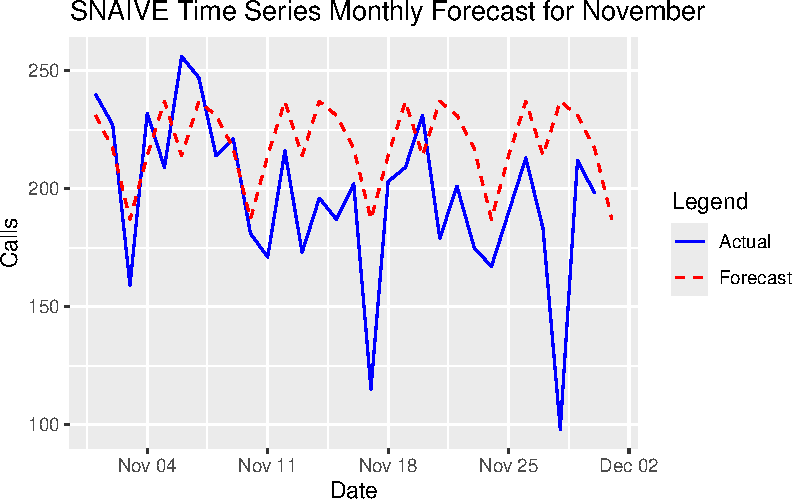
\includegraphics{final_proj_group1_files/figure-pdf/unnamed-chunk-23-1.pdf}

\begin{Shaded}
\begin{Highlighting}[]
\CommentTok{\# visualization of the errors}
\NormalTok{errors\_viz }\OtherTok{\textless{}{-}} \FunctionTok{ggplot}\NormalTok{(nov\_results, }\FunctionTok{aes}\NormalTok{(}\AttributeTok{x =}\NormalTok{ Date)) }\SpecialCharTok{+} 
  \FunctionTok{geom\_line}\NormalTok{(}\FunctionTok{aes}\NormalTok{(}\AttributeTok{y =}\NormalTok{ Error, }\AttributeTok{color =} \StringTok{"Error"}\NormalTok{, }\AttributeTok{linetype =} \StringTok{"Error"}\NormalTok{)) }\SpecialCharTok{+}
  \FunctionTok{labs}\NormalTok{(}\AttributeTok{title =} \StringTok{"SNAIVE Time Series Monthly Forecast Errors for November"}\NormalTok{,}
       \AttributeTok{x =} \StringTok{"Date"}\NormalTok{,}
       \AttributeTok{y =} \StringTok{"Error"}\NormalTok{,}
       \AttributeTok{color =} \StringTok{"Legend"}\NormalTok{,}
       \AttributeTok{linetype =} \StringTok{"Legend"}\NormalTok{)}

\NormalTok{errors\_viz}
\end{Highlighting}
\end{Shaded}

\begin{verbatim}
Warning: Removed 1 row containing missing values or values outside the scale range
(`geom_line()`).
\end{verbatim}

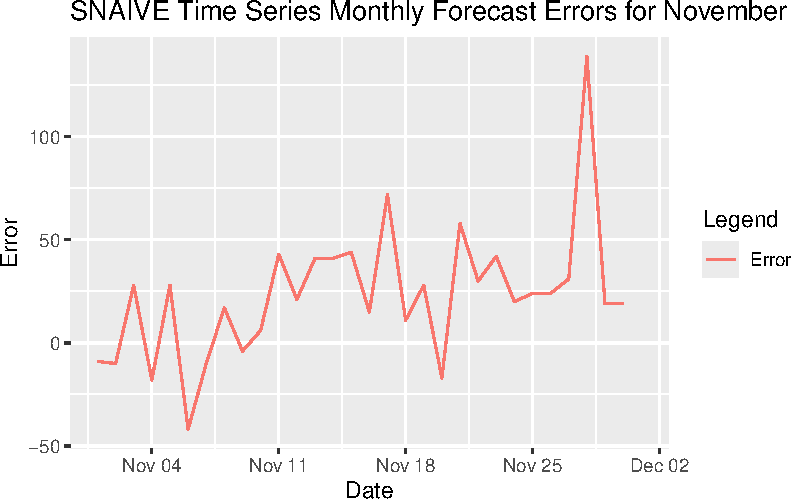
\includegraphics{final_proj_group1_files/figure-pdf/unnamed-chunk-24-1.pdf}




\end{document}
